%%%%%%%%%%%%%%%%%%%%%%%%%%%%%%%%%%%%%%%%%%%%%%%%%%%%%%%%%%%%%%%%%%%%%%%%%%%%%%%%%%%%%%%%%%%%%%%%%%%%%%%%%%%%%%%%%%%%%%%%%%%%%%%%%%%%%%%%%%%%%%%%%%%%%%%%%%%
% This is just an example/guide for you to refer to when submitting manuscripts to Frontiers, it is not mandatory to use Frontiers .cls files nor frontiers.tex  %
% This will only generate the Manuscript, the final article will be typeset by Frontiers after acceptance.   
%                                              %
%                                                                                                                                                         %
% When submitting your files, remember to upload this *tex file, the pdf generated with it, the *bib file (if bibliography is not within the *tex) and all the figures.
%%%%%%%%%%%%%%%%%%%%%%%%%%%%%%%%%%%%%%%%%%%%%%%%%%%%%%%%%%%%%%%%%%%%%%%%%%%%%%%%%%%%%%%%%%%%%%%%%%%%%%%%%%%%%%%%%%%%%%%%%%%%%%%%%%%%%%%%%%%%%%%%%%%%%%%%%%%

%%% Version 3.4 Generated 2018/06/15 %%%
%%% You will need to have the following packages installed: datetime, fmtcount, etoolbox, fcprefix, which are normally inlcuded in WinEdt. %%%
%%% In http://www.ctan.org/ you can find the packages and how to install them, if necessary. %%%
%%%  NB logo1.jpg is required in the path in order to correctly compile front page header %%%

\documentclass[utf8]{frontiersSCNS} % for Science, Engineering and Humanities and Social Sciences articles
%\documentclass[utf8]{frontiersHLTH} % for Health articles
%\documentclass[utf8]{frontiersFPHY} % for Physics and Applied Mathematics and Statistics articles

%\setcitestyle{square} % for Physics and Applied Mathematics and Statistics articles
\usepackage{url,hyperref,lineno,microtype,subcaption}
\usepackage[onehalfspacing]{setspace}

%%% --- added by Matthias ---
\usepackage{tabularx}  % controls the table width
\usepackage{booktabs}

\usepackage{multirow}
\usepackage{prettyref}
\usepackage{amsmath}
\usepackage[dvipsnames]{xcolor}
\usepackage{bbm}    % for 1 as a vector

\graphicspath{{figures/}}

\newcommand{\todo}[1]{\textcolor{Magenta}{todo: #1}}
\newcommand{\red}[1]{\textcolor{Red}{#1}}
\newcommand{\mt}[1]{\textcolor{SeaGreen}{mt: #1}}
\newcommand{\kt}[1]{\textcolor{Red}{kt: #1}}
\newcommand{\fk}[1]{\textcolor{Periwinkle}{fk: #1}}
\newcommand{\js}[1]{\textcolor{RedOrange}{js: #1}}

\newrefformat{fig}{Figure \ref{#1}}
\newrefformat{tab}{Table \ref{#1}}
\newrefformat{eq}{Eq. (\ref{#1})}
\newrefformat{app}{Appendix \ref{#1}}
\newrefformat{sec}{Section \ref{#1}}
\newrefformat{lemma}{Lemma \ref{#1}}
\newrefformat{theorem}{Theorem \ref{#1}}
\newrefformat{assumption}{Assumption \ref{#1}}

% Math symbols
\renewcommand{\a}{\theta} 
% \renewcommand{\a}{a} 
\newcommand{\az}{\a_0} 
\newcommand{\ar}{\a_\rho} 
\newcommand{\al}{\boldsymbol{\alpha}}
\newcommand{\ah}{\widehat{\boldsymbol{\alpha}}}
\renewcommand{\b}{\boldsymbol{\beta}} % true beta
\newcommand{\bO}{\boldsymbol{\beta}_0} % true beta
\newcommand{\bh}{\boldsymbol{\hat{\beta}}} % estimate
\newcommand{\bcc}{\boldsymbol{\hat{\beta}}_\text{cc}} % estimate
\newcommand{\bOLS}{\boldsymbol{\hat{\beta}}_\text{ols}}
\newcommand{\corr}{\text{corr}}
\renewcommand{\d}{\boldsymbol{\delta}}
\newcommand{\e}{\mathbf{e}}
\newcommand{\eps}{\boldsymbol{\epsilon}}
\renewcommand{\H}{\mathbf{H}}
\newcommand{\I}{\mathbf{I}}
\newcommand{\K}{\mathbf{K}}
\renewcommand{\L}{\mathcal{L}}
% \newcommand{\mx}{\mathbf{m_x}}
\newcommand{\mx}{\mathbf{\bar{x}}}
\newcommand{\my}{\bar{y}}
% \newcommand{\my}{m_y}
\newcommand{\N}{\mathcal{N}}   % normal distribution
\newcommand{\one}{\mathbf{1}} 
\newcommand{\R}{\mathbb{R}}
\newcommand{\x}{\mathbf{x}}
\newcommand{\X}{\mathbf{X}}
\newcommand{\yhat}{\hat{y}}
\newcommand{\y}{\mathbf{y}}
\newcommand{\yc}{\mathbf{y}_c}
\newcommand{\yh}{\mathbf{\hat{y}}}
\newcommand{\yhc}{\mathbf{\hat{y}}_c}
\newcommand{\yOLS}{\mathbf{\hat{y}}_\text{OLS}}
\newcommand{\yridge}{\mathbf{\hat{y}}_\text{ridge}}
\newcommand{\yt}{\mathbf{\widetilde{y}}}
\newcommand{\z}{\mathbf{z}}

\linenumbers



% Leave a blank line between paragraphs instead of using \\


\def\keyFont{\fontsize{8}{11}\helveticabold }
\def\firstAuthorLast{Treder {et~al.}} %use et al only if is more than 1 author
\def\Authors{Matthias S. Treder\,$^{1,*}$, Jonathan P. Shock\,$^{2}$, Dan J. Stein\,$^{3}$, Stefan DuPlessis\,$^{4}$,  Soraya Seedat\,$^{4}$, \& Kamen A. Tsvetanov\,$^{5,6}$}
% Affiliations should be keyed to the author's name with superscript numbers and be listed as follows: Laboratory, Institute, Department, Organization, City, State abbreviation (USA, Canada, Australia), and Country (without detailed address information such as city zip codes or street names).
% If one of the authors has a change of address, list the new address below the correspondence details using a superscript symbol and use the same symbol to indicate the author in the author list.
\def\Address{$^{1}$School of Computer Science \& Informatics, Cardiff University, Cardiff, United Kingdom\\$^{2}$Department of Mathematics and Applied Mathematics, University of Cape Town, Cape Town, South Africa\\$^{3}$SA MRC Unit on Risk \& Resilience in Mental Disorders, Department of Psychiatry and Neuroscience Institute, University of Cape Town, Cape Town, South Africa\\$^{4}$Department of Psychiatry, Faculty of Medicine and Health Sciences, Stellenbosch University, Cape Town, South Africa\\$^{5}$Department of Clinical Neurosciences, University of Cambridge, United Kingdom\\$^{6}$Department of Psychology, University of Cambridge, United Kingdom}

% The Corresponding Author should be marked with an asterisk
% Provide the exact contact address (this time including street name and city zip code) and email of the corresponding author
\def\corrAuthor{Corresponding Author}

\def\corrEmail{trederm@cardiff.ac.uk}




\begin{document}
\onecolumn
\firstpage{1}

\title[Correlation-constrained regression]{Correlation constraints for regression models: controlling bias in brain age prediction} 

\author[\firstAuthorLast ]{\Authors} %This field will be automatically populated
\address{} %This field will be automatically populated
\correspondance{} %This field will be automatically populated

\extraAuth{}% If there are more than 1 corresponding author, comment this line and uncomment the next one.
%\extraAuth{corresponding Author2 \\ Laboratory X2, Institute X2, Department X2, Organization X2, Street X2, City X2 , State XX2 (only USA, Canada and Australia), Zip Code2, X2 Country X2, email2@uni2.edu}


\maketitle


\begin{abstract}

%%% Leave the Abstract empty if your article does not require one, please see the Summary Table for full details.
% \section{}
In neuroimaging, the difference between chronological age and predicted brain age, also known as \textit{brain age delta}, has been proposed as a pathology marker linked to a range of phenotypes. Brain age delta is estimated using supervised-learning algorithms (e.g. regression), which involves a frequently observed bias due to a negative correlation between the chronological and brain age delta. In brain age prediction models, this correlation can manifest as an overprediction of the age of young brains and an underprediction for elderly ones. We show that this bias can be controlled for by adding correlation constraints to the model fitting procedure.
We develop an analytical solution to this constrained optimization problem for linear, ridge, and kernel ridge regression. The solution is optimal in the least-squares sense i.e. there is no other model that satisfies the correlation constraints and has a better fit. 
%We also show to harness our findings in more complex approaches such as convolutional neural networks. 
Analyses on the PAC2019 competition data demonstrate that this approach produces optimal unbiased predictive models with a number of advantages over existing approaches. 
Finally, we introduce regression toolboxes for MATLAB and Python that implement our algorithm.

\tiny
 \keyFont{\section{Keywords:} regression, correlation, prediction, brain, age} %All article types: you may provide up to 8 keywords; at least 5 are mandatory.
\end{abstract}

\section{Introduction}

As the world’s population ages, early detection and prevention of neurological aspects of aging, such as cognitive decline and dementia, is a public health priority and challenge. Pathological aging could be indicated by the level of deviation from the typical pattern of aging in healthy individuals \citep{Cole2018BrainMortality}. There has been growing interest in developing statistical approaches in order to identify individuals deviating from a healthy brain aging trajectory \citep{Cole2017PredictingBiomarker}. To this end, a metric referred to as \textit{brain age delta}, defined as the difference between brain-predicted age and chronological age, has been proposed as an index of the level of neuropathology in aging \citep{Cole2017PredictingBiomarker,Smith2019EstimationImaging,deLange2020Commentary:Prediction}. Investigating the association between this metric with demographics, and lifestyle and cognitive variables can deepen the understanding of the processes that underpin healthy aging  \citep{Borgeest2020GreaterAbilities}. In clinical research, brain age delta has the potential to index the severity of premature aging in patients suffering from disease. Among others, a higher delta has been associated with lower fluid intelligence and higher mortality \citep{Cole2018BrainMortality}, risk for developing Alzheimer’s disease \citep{Gaser2013BrainAGEDisease}, severity of schizophrenia and depression  \citep{Koutsouleris2014AcceleratedDisorders}.


% METHODOLOGICAL CHALLENGES
Establishing a good estimate of brain age delta is faced with important methodological challenges. The first challenge relates to the kinds of features (biomarkers) and predictive models that are used to build a brain-age model. A number of brain metrics have been considered as features for regression models; for example, structural networks \citep{Jiang2020PredictingNetworks}, cortical thickness \citep{Aycheh2018BiologicalStudy}, functional connectivity patterns \citep{Zhai2019PredictingNetworks,Monti2020InterpretableConnectivity}, and raw T1-weighted images \citep{Cole2017PredictingBiomarker,Cole2018BrainMortality}. Likewise, a variety of regression models has been tested, from linear regression models such as lasso and support vector regression \citep{Zhai2019PredictingNetworks,Monti2020InterpretableConnectivity} to convolutional neural networks (CNNs; \citep{Cole2017PredictingBiomarker,Jiang2020PredictingNetworks}).
The quest for more accurate brain-age models lied at the heart of the Predictive Analytics Competition (PAC) 2019 upon which the eponymous Frontiers Research Topic is founded\footnote{www.frontiersin.org/research-topics/13501/predicting-chronological-age-from-structural-neuroimaging-the-predictive-analytics-competition-2019}.

A more fundamental methodological challenge, and the starting point for this paper, is the very operationalization of the brain age delta. If we denote the chronological age for a set of participants as a vector $\y$, the ages predicted on the brain scans as $\yh$, and the residuals as $\e = \y - \yh$, then the negative residual $\d = -\e$ (i.e. predicted brain age minus chronological age) is usually defined as the brain age delta. This metric has been shown to be problematic. A predictive bias manifesting as an overprediction of the age of young individuals and an underprediction for elderly individuals has led to much speculation and investigation  \citep{Aycheh2018BiologicalStudy,Beheshti2019Bias-adjustmentScheme,Cole2017PredictingBiomarker,Cole2015PredictionInjury,Le2018ABrainAGE,Liang2019InvestigatingDisorders,Smith2019EstimationImaging}. 

A useful quantification of this effect is the correlation between chronological age and delta, corr($\y, \d$), which we will refer to as \textit{age delta correlation (ADC)} in the rest of the paper. An analysis by \cite{Liang2019InvestigatingDisorders} showed that negative ADC is ubiquitous across a range of aging datasets and regression models and independent of the age range included in the dataset. A theoretical analysis by  \cite{Le2018ABrainAGE} showed that this effect is an inevitable property of regression, further aggravated by regression dilution \citep{Fuller1987MeasurementModels,MacMahon1990BloodBias}, and hence not limited to aging data. The potential danger of non-zero ADC lies in spurious associations with other covariates: brain age delta can be trivially correlated with demographic or cognitive variables if the latter are correlated with chronological age as well. \cite{Le2018ABrainAGE} found that associations between residuals and variables obtained from  clinical interviews and neuropsychological testing largely disappear when residuals are corrected for chronological age. To avoid these spurious correlations, several authors have suggested following up the regression analysis with a correction step wherein the effect of age is removed from the residuals \citep{Le2018ABrainAGE,Smith2019EstimationImaging,Beheshti2019Bias-adjustmentScheme}. Brain age delta is then calculated by the following two-stage approach:

\begin{enumerate}
    \item \textit{Brain age prediction.} Train a regression model to predict age from neuroimaging data. The difference between predicted age and chronological age reflects \textit{uncorrected brain age delta}.
    \item \textit{Correction of brain age delta.}
    Use simple linear regression to regress delta against age. The resultant residuals are uncorrelated with age and denoted as \textit{corrected brain age delta}. 
\end{enumerate}

% AIM
\mt{Despite the significant methodological progress that has been made there are still methodological concerns that warrant attention. First, the correction approach is an ad hoc fix because the models' predictions do not take ADC into account. Second, in a strictly sequential two-stage approach it is not clear whether the resultant brain age delta is optimal in terms of predictive accuracy. Both issues can be addressed when prediction and correction are unified within a model. Third, in predictive settings with training and test set, zeroing ADC on the training set is not of primary importance. 
Rather, it would be useful to have a model that is able to finely control the trade-off between ADC and predictive performance.} 

The aim of this study was to address these points by introducing modifications on three different regression models (Linear, Ridge and Kernel Ridge regression). Our models explicitly control for ADC on the training set without the need for an additional correction after model training. This was realized by formulating constrained optimization problems that incorporate age delta correlation as additional constraints. Our approach offers the following features: 

\begin{itemize}
    \item\textit{Predictive model.} In predictive modeling, all properties of the estimation pipeline (including correction of the residuals) should be derived from the training set and validated on an independent test set. Some of the existing approaches conflate training and test data because age prediction is based on the training data but the correction is performed on the test set. This introduces dependencies between test samples and violates the assumptions of predictive models.
    \item \textit{Arbitrary test set size.} An additional problem arising from conflating training and test sets is that performing correction on test data requires a sufficiently large test set. This is especially problematic with smaller datasets because fewer data are available for training. Since our approach estimates all parameters from the training data, it can be applied with any train/test split including leave-one-out cross-validation, when appropriate.
    \item \textit{Prediction of unlabeled data.} Our model corrects the predictions not the residuals. Therefore, corrected predictions can be obtained even on unlabeled data if necessary.
    \item \textit{Optimality.} Formulating both model training and correction as a single constrained optimization problem allowed us to show that the resultant models are optimal in terms of mean-squared error (MSE) on the training set. In other words, of all potential solutions that control ADC, our solution has the highest accuracy on the training data.
    \item\textit{Correlation bounds.} Our models allow for 'soft' control of the ADC by setting a cap on the maximum permissible correlation, e.g. $|\corr(\y,\d)|\le 0.1$. This is especially useful for predictive modeling, because minimizing age delta correlation on the training set is not vital. Rather, a low bias and good predictive performance on the test set is desired. Using correlation bounds, our models allow for fine-tuning of the trade-off between ADC and predictive accuracy.
\end{itemize}

Some of the existing approaches share some of the listed features. For instance, whereas in \cite{Le2018ABrainAGE} test set residuals are used for correction,  \cite{Beheshti2019Bias-adjustmentScheme} learns the correction parameters from the training set and applies them to the test set, in line with good practice for predictive models. 
However, to the best of our knowledge, this is the first study to prove optimality of the models and introduce 'soft' correlation bounds for fine control of ADC.


The Methods section is organized as follows. In \prettyref{sec:current_approaches} we review existing ways to quantify brain age delta. In \prettyref{sec:regression_models} we introduce Linear regression, Ridge regression and Kernel Ridge regression. In \prettyref{sec:ADC}, we revisit the mathematical basis for ADC in the context of these three regression models. In \prettyref{sec:correlation_constraints} we develop our approach by adding correlation constraints to the model training stage that allow for a precise control of ADC. In \prettyref{sec:relationship} it is shown that the brain age estimates obtained with our models are closely related to existing correction approaches. 
In \prettyref{sec:toolbox} we introduce toolboxes for Python and MATLAB that implement our models. Finally, in \prettyref{sec:neuroimaging} and \prettyref{sec:brain_age_prediction} we describe our analysis of the PAC2019 competition data. 


%%%%%%%%%%%%%%%%%%%%%%
%%%%%%%%%%%%%%%%%%%%%%
%%      METHOD      %%
%%%%%%%%%%%%%%%%%%%%%%
%%%%%%%%%%%%%%%%%%%%%%
\section{Method}
\subsection{Notation}

\begin{table}[htbp]\caption{Mathematical notation, dimensionality, and description for the main quantities used in the regression models.}
\begin{center}% used the environment to augment the vertical space
% between the caption and the table
\begin{tabular}{r c p{10cm} }
\toprule
$n$ &  & Number of samples\\
$p$ &  & Number of features\\
$\b$ & $\R^p$ & Regression coefficients ($\b=[\beta_1,\beta_2,...,\beta_p]^\top$)\\
$\X$ & $\R^{n\times p}$ & Brain scans (features)\\
$\y$ & $\R^n$ & Chronological age (targets)\\
$\yh$ & $\R^n$ & Predicted age ($\yh = \X\b$)\\
$\e$ & $\R^n$ & Residuals ($\e=\y - \yh$) \\
$\d$ & $\R^n$ & Brain-age delta (negative residuals $\d =-\e$)\\
\midrule
$\top$ &  & Transpose operator\\
$\one$ & $\R^n$ & Vector of 1's\\
$\mx$ & $\R^p$ & Column means of $\X$ given by $\frac{1}{n}\X^\top\one$\\
$\my$ & & Mean of $y$\\
\bottomrule
\end{tabular}
\end{center}
\label{tab:notation}
\end{table}

\prettyref{tab:notation} defines the most important mathematical symbols used in the paper. Whenever the symbol represents a vector or matrix, its dimensionality is given in the second column. In general,  matrices are denoted as uppercase boldface symbols (e.g. $\X$, $\H$), vectors as lowercase boldface symbols (e.g. $\b$, $\mx$), and scalars as lowercase normal face symbols (e.g. $n, \beta_0, \my$). Note that we use terminology common in the machine learning literature. In particular, \textit{features} are also known as predictors or independent variables in the regression literature, and the vector of \textit{targets} (chronological age) is also known as response vector or dependent variable. 
If an intercept is included in the model, we assume that a column of 1's is added to $\X$ and an entry for the intercept coefficients is added to $\b$, although sometimes we will denote the intercept separately as $\beta_0$.

%We denote as $\X\in\R^{n\times p}$ the matrix of features (a.k.a. predictors or independent variables) with $n$ samples and $p$ features. Let $\y\in\R^n$ be the vector of targets (a.k.a. responses or dependent variable) and $[\beta_1,\beta_2,...,\beta_p]^\top=\b\in\R^p$ the vector of regression weights. If an intercept is included in the model, we assume that a column of 1's is added to $\X$ and an entry for the intercept coefficients is added to $\b$. Sometimes we will denote the intercept separately by the symbol $\beta_0$. The predicted responses are denoted as the vector $\yh := \X\b$. The vector of  residuals is given by $\e := \y - \yh$. Let $\mx=\frac{1}{n}\X^\top\one\in\R^p$ be the vector of column means of $\X$, $\my=\frac{1}{n}\y^\top\one\in\R$ the mean of $\y$, and $\one\in\R^n$ a vector of 1's. 

\subsection{Calculating the brain-age delta}\label{sec:current_approaches}

The regression of age on brain features often leads to a biased model that manifests as an overprediction of the age of younger individuals and an underprediction of the age of elderly ones. This effect can be quantified as a negative age delta correlation (ADC) denoted as $\corr(\y,\d)$. In the literature, ADC has been set to zero by adding a second stage to the analysis wherein the regression predictions from the first stage are corrected. Hence, brain-age delta prediction can be formulated as the following two-stage approach:

\begin{enumerate}
    \item[(a)]\textit{Training the regression model.} Train a regression model $f$ to predict age such that $\y \approx f(\X)$. The negative residuals, denoted as 
    \begin{equation}\label{eq:twostage1}
         \d = f(\X) - \y
    \end{equation}
    represent the (uncorrected) brain age delta. 
\end{enumerate}

A number of authors proposed correction procedures to rid $\d$ of ADC  \citep{Le2018ABrainAGE,Smith2019EstimationImaging,Beheshti2019Bias-adjustmentScheme}. These approaches turned out to be mathematically equivalent and boil down to the following operation:
    
\begin{enumerate}
    \setcounter{enumi}{1}
    \item[(b)]\textit{Approach 1: Correction of residuals.} Train a simple regression model $\d\approx\y\beta_1 + \beta_0$ to remove the linear effect of age from the delta estimate. The new estimate
    \begin{equation}\label{eq:approach1_d}
         \d_1 = \d - \y\beta_1 - \beta_0
    \end{equation}
    represents corrected brain age delta which is uncorrelated with age.
\end{enumerate}

As an alternative approach, it has been suggested that $\yh$ instead of $\d$ be used in the regression  \citep{Cole2018BrainMortality,deLange2020Commentary:Prediction} and then a correction made for the predictions:

\begin{enumerate}
    \setcounter{enumi}{1}
    \item[(b')]\textit{Approach 2: Correction of predictions.} Train a simple regression model $\yh\approx\y\beta_1 + \beta_0$. Then define corrected predictions $\yh_2$ as 
    \begin{equation}\label{eq:approach2_y}
         \yh_2 = \frac{\yh - \beta_0}{\beta_1}
    \end{equation}
    with corresponding brain age delta
    \begin{equation}\label{eq:approach2_d}
         \d_2 = \yh_2 - \y.
    \end{equation}
\end{enumerate}

The residuals calculated based on the modified predictions are again uncorrelated with age. The relationship between these two approaches and our zero correlation constraint (\prettyref{sec:zero_correlation_constraint}) is investigated in \prettyref{sec:relationship}.

%The aim of our approach presented in the next subsections is to introduce Linear, Ridge, and Kernel Ridge regression models that perform training and correction internally, and that give control over the maximum permissible correlation. In \prettyref{sec:relationship}, we investigate the special case of a zero correlation constraint. Our approach then yields the same predictions as approach 2' \citep{Cole2018BrainMortality,deLange2020Commentary:Prediction}. Furthermore, both approaches 2 and 2' yield brain age delta estimates that differ by a well defined scaling factor $\a$ defined in \prettyref{eq:scaling_factor}.

\subsection{Regression models}\label{sec:regression_models}

\subsubsection{Ordinary least-squares (OLS) regression}

Ordinary least-squares regression, often just called linear regression, can be formulated as a set of $n$ equations of the form

\[
y_i = \beta_0 + \beta_1 x_{i1}+ \beta_2 x_{i2} + ... + \beta_p x_{ip} + \epsilon_i\quad\quad i=1, 2, ..., n
\]

where $y_i$ is the $i$-th response, $x_{ij}$ is the $j-th$ predictor value in the $i$-th sample, the $\beta$'s are regression coefficients, and  $\epsilon\sim\N(0,\sigma^2)$ is an error term. Using matrix notation, this set of equations can be written more succinctly as:

\begin{equation}\label{eq:linear_regression}
\y = \X\b + \eps
\end{equation}

where $\y=[y_1, y_2, ..., y_n]^\top$ comprises the responses, $\X\in\R^{n\times p}$ is the matrix of predictors, $\b\in\R^p$ is the vector of regression coefficients and 
$\eps=[\epsilon_1,\epsilon_2,...,\epsilon_n]^\top$ collects all error terms. Fitting a model implies finding an estimate $\bh$ such that $\y\approx\X\bh$. In OLS regression this is achieved by minimizing the sum of squared errors $||\y-\X\b||_2^2$. Denoting $\yh := \X\bh$ this can be formulated as the unconstrained optimization problem

\begin{equation}\label{eq:ols_optimization_problem}
\text{minimize}\quad ||\y-\yh||_2^2.
\end{equation}

 The solution is given by 
 
 \begin{equation}\label{eq:ols_solution}
 \bOLS =(\X^\top\X)^{-1}\,\X^\top\y.
 \end{equation}

\subsubsection{Ridge regression}

OLS regression suffers from high bias and does not have a unique solution if the number of the predictors $p$ is larger than the number of samples $n$ \citep{Marquardt1975RidgePractice,vanWieringen2015LectureRegression}. Ridge regression is a regularized version of OLS regression that is useful for data that suffers from multicollinearity. The model is regularized by adding a $\ell_2$ penalty that shrinks the weights towards zero. For a given regularization parameter $\lambda\ge0$, ridge regression can be formulated as the following unconstrained optimization problem

\begin{equation*}
\text{minimize}\quad ||\y-\yh||_2^2 + \lambda ||\b||_2^2.
\end{equation*}

The first term is the least-squares term from \prettyref{eq:ols_optimization_problem}. The second term penalizes elements of $\bh$ from becoming too large. For $\lambda=0$ ridge regression reduces to OLS regression. The solution is given by

\begin{align}
\label{eq:ridge_solution}
\bh_\text{ridge} =\ & (\X^\top\X + \lambda\I)^{-1}\ \X^\top\y 
\end{align}

where $\I\in\R^{p\times p}$ is an identity matrix.  Note that the intercept term is not regularized. That is, if the model contains an intercept, $\I$ is modified such that the 1 in the respective row is replaced by a 0.


\subsubsection{Other linear regression models}

Other variants of linear regression e.g. lasso \citep{Tibshirani1996RegressionLasso} and elastic net \citep{Zou2005RegularizationNet}, do not have a closed form solution but rely on iterative optimization, so they do not lend themselves to the analytical approach developed in this paper.

\subsubsection{Kernel ridge regression (KRR)}

A non-linear version of ridge regression can be developed by applying a non-linear transformation to the predictors and then performing ridge regression on these transformed predictors \citep{Hainmueller2014KernelApproach}. Let this transformation be represented by a map $\phi:\R^p\rightarrow\mathcal{F}$ from input space to a higher-dimensional Reproducing Kernel Hilbert Space and $\Phi(\X) = [\phi(\x_1),\phi(\x_2),...,\phi(\x_n)]^\top$ \citep{Scholkopf2003AKernels,Hofmann2008}. The solution is given by replacing $\X$ by $\Phi(\X)$ in \prettyref{eq:ridge_solution},

\begin{align*}
%\label{eq:kernel_ridge_primal_solution}
\bh_\text{krr} =\ (\Phi(\X)^\top\Phi(\X) + \lambda\I)^{-1}\ \Phi(\X)^\top\y.
\end{align*}

This solution, also known as primal solution, is of limited practical use, since the feature space is too high-dimensional to represent $\bh_\text{krr}$ and $\Phi(\X)$. As an alternative, the convex optimization problem can be rewritten into its dual Lagrangian form first  
\citep{Bishop2007}. The resultant dual solution is given by

\begin{align}
\label{eq:kernel_ridge_dual_solution}
\bh_\text{krr}  =\ \Phi(\X)^\top (\Phi(\X)\Phi(\X)^\top + \lambda\I)^{-1}\ \y.
\end{align}


The equivalence between the primal and dual solution can be verified by left-multiplying both solutions with $(\Phi(\X)\Phi(\X)^\top + \lambda\I)$. Since $\bh_\text{krr}$ cannot be represented directly, we instead calculate a vector of dual weights $\al\in\R^n$. To this end, define $\K = \Phi(\X)\,\Phi(\X)^\top$ as the kernel matrix with $\K_{ij} = k(\x_i, \x_j)$ for a kernel function $k$. Then the vector of dual weights is given by the latter part of \prettyref{eq:kernel_ridge_dual_solution}, 

\begin{align}
\begin{split}
\label{eq:kernel_ridge}
\al = (\K + \lambda\I)^{-1}\ \y.
\end{split}
\end{align}

Using $\al$ the predicted response to a test sample $\x$ can be rewritten in terms of kernel evaluations:

\begin{align}
\begin{split}
\label{eq:kernel_ridge_apply}
f(\x) = \b_\phi^\top\, \phi(\x) = \al^\top\Phi(\X)\,\phi(\x) = \sum_{i=1}^n \al_i\, k(\x_i, \x).
\end{split}
\end{align}

%%%%%%%%%%%%%%%%%%%%%%
%%  PREDICTION BIAS %%
%%%%%%%%%%%%%%%%%%%%%%

\subsection{Negative age delta correlation (ADC)}\label{sec:ADC}

The theoretical basis for negative ADC has already been discussed in \cite{Le2018ABrainAGE}. In particular, the authors highlighted that ADC $\le 0$ for any sensible regression model. Here, we discuss ADC more specifically for the three regression models introduced above. To start, we will address OLS regression. Let us expand the age delta correlation term as

\begin{equation}\label{eq:correlation}
\corr(\y,\d) = \frac{\y^\top(\yh-\y)}{||\y||\ ||\yh-\y||} 
\end{equation}

where to simplify the notation we assume that $\X$ and $\y$ have been centered. The sign of the correlation is determined by the numerator. Using the identity $\yh = \H\y$ we obtain

\begin{equation}\label{eq:tmp}
\begin{split}
- \y^\top\y + \y^\top\H\,\y = -  \y^\top(\I-\H)\,\y\le 0
\end{split}
\end{equation}

where the inequality follows from the fact that  $\I-\H$ is symmetric and idempotent and therefore positive semi-definite \citep{Draper1966AppliedAnalysis}. This implies that the ADC is always non-positive in OLS regression.
Ridge regression coincides with OLS regression 
for $\lambda=0$. As  $\lambda$ increases, $\b$ tends to zero due to the shrinkage effect of the regularization \citep{Marquardt1975RidgePractice}. This implies that $\yh\rightarrow 0$ and therefore $\text{corr}(\y,\d)\rightarrow -1$ as $\lambda$ increases. This is illustrated empirically in \prettyref{fig:ADC}c. The same argumentation holds for kernel ridge, one only has to replace $\X$ by $\Phi(\X)$. Often, kernel ridge models will have a smaller prediction bias because their higher complexity allows for a better fit to the data. In line with previous work, this suggests that a negative ADC is nearly inevitable and that regularization further exacerbates this effect \citep{Le2018ABrainAGE,Smith2019EstimationImaging}.

%%%%%%%%%%%%%%%%%%%%%%%%%%%%%%%%%%%%%
%%     CORRELATION CONSTRAINTS     %%
%%%%%%%%%%%%%%%%%%%%%%%%%%%%%%%%%%%%%
\subsection{Correlation constraints for regression}\label{sec:correlation_constraints}


The regression problems defined in \prettyref{sec:regression_models} can be cast as  unconstrained optimization problems. The optimization involves the minimization of a \textit{loss function} $\L$ which measures the amount of discrepancy between the true responses $\y$ and the model predictions $\yh$:

\begin{equation}\label{eq:unconstrained_problem}
\begin{split}
    % \underset{\b}{\text{minimize}}\quad \L(y_i,\yhat_i)   
    \text{minimize}\quad \L(\y,\yh).
\end{split}
\end{equation}

In OLS regression the loss function is the squared loss $\L(\y,\yh)=||\y-\yh||_2^2$ whereas it is $\L(\y,\yh)=||\y-\yh||_2^2 + \lambda||\b||_2$ in ridge and kernel ridge regression. To control for age delta correlation at the level of training, we can add a correlation constraint that caps the permitted magnitude of correlation between the brain age delta and age. To this end, consider the constrained optimization problem

\begin{equation}\label{eq:constrained_problem_bounded}
\begin{split}
    \text{minimize}\quad& \L(\y,\yh)\\
\text{subject to}\quad&   |\corr(\y,\d)| \le \rho.
\end{split}
\end{equation}

In this problem, the same loss function as before is minimized. However, the set of feasible solutions is limited to solutions for which the absolute value of the correlation does not exceed $\rho$, where $\rho\ge0$ is a threshold value selected by the user. As a special case of \prettyref{eq:constrained_problem_bounded}, we can consider the case $\rho=0$, that is, the responses have to be perfectly uncorrelated with the residuals: 

\begin{equation}\label{eq:constrained_problem_zero}
\begin{split}
    \text{minimize}\quad& \L(\y,\yh)\\
    \text{subject to}\quad&  \corr(\y,\d) = 0.
\end{split}
\end{equation}

We will address the latter case first and see that it leads to a simple solution. In the following, we will assume that $\X$ and $\y$ have been centered and the model contains no intercept since this simplifies the equations.  This does not limit the generality of our results. As shown in \prettyref{app:equal_coefficients}, a model with centered data and without intercept yields the same regression coefficients as a model with intercept. In other words, we can first calculate $\b$ on the centered data and subsequently calculate the intercept $\beta_0$ to obtain the model for non-centered data.



% By extending the loss function with regularization terms, other techniques such ridge regression, lasso, and elastic net, can be derived:

% % \begin{equation}
% \begin{alignat*}{2}% \begin{split}
%   &\L(\y,\yh) = \sum_{i=1}^n |\y_i - \yh_i|^2 \quad&\text{(OLS regression)}\\
%   &\L(\y,\yh) = \sum_{i=1}^n |\y_i - \yh_i|^2 + \lambda\,||\b||_2 \quad&\text{(ridge regression)}\\
%   &\L(\y,\yh) = \sum_{i=1}^n |\y_i - \sum_j \alpha_j k(\x_j,\x_i)|^2 \quad&\text{(kernel ridge)}\\
%   &\L(\y,\yh) = \sum_{i=1}^n |\y_i - f(\x_i)|^2 \quad&\text{(CNN with MSE loss)}\\
%   %   &\L(\y,\yh) = \sum_{i=1}^n |\y_i - \yh_i|^2 + \lambda\,||\b||_1 \quad&\text{(lasso)}\\
% %   &\L(\y,\yh) = \sum_{i=1}^n |\y_i - \yh_i|^2+\lambda_1\,||\b||_1+\lambda_2\,||\b||_2 \quad&\text{(elastic net)}% \end{split}\
% \end{alignat*}
% % \end{equation}

% where $||\cdot||_1$ and $||\cdot||_2$ represent $\ell_1$ and $\ell_2$ norms, respectively, and the $\lambda$'s are regularization hyperparameters. For OLS and ridge regression, the regression coefficients are given by


\subsubsection{Zero correlation constraint}\label{sec:zero_correlation_constraint}

A hard correlation constraint can be set that requires the correlation between the residuals and the response values to be zero, that is $|\corr(\y,\d)|=0$. In \prettyref{app:solution_zero_correlation} the optimal solution, $\bcc$, is derived for OLS, ridge and kernel ridge regression. It is given as a scaled version of the standard, unconstrained solution

\begin{equation}
 \bcc = \az\, \bh
\end{equation}

where $\bh$ is the standard OLS, ridge or kernel ridge solution and it is assumed that $\X$ and $\y$ have been centered. The scaling factor $\az$ is given by

\begin{equation}\label{eq:scaling_factor}
 \az = \frac{||\y||^2}{\y^\top\H\y}
\end{equation}

with model-specific hat matrices $\H$:

\begin{equation*}
\begin{split}
\H =&\ \X\,(\X^\top\X)^{-1}\,\X^\top\quad \text{(OLS)}\\
\H =&\ \X\,(\X^\top\X + \lambda\I)^{-1}\,\X^\top  \quad\text{(ridge)}\\
\H =&\ \K\,(\K + \lambda\I)^{-1}\quad\text{(kernel ridge)}.
\end{split}
\end{equation*}

\textit{Intercept term}: If the data has not been centered and the model includes an intercept term, $\y$ and $\y^\top\H\y$ need to be centered before calculating $\a$. The intercept $\b_0$ can be obtained from the equation

\begin{equation*}
\begin{split}
(\y - \one\, \my) =&\  (\X - \one\,\mx^\top)\ \bcc\\
\Leftrightarrow\ \y =&\ \X\bcc + \one\,(\my - \mx^\top\bcc)
\end{split}
\end{equation*}


from which it follows that $\beta_0 = \my - \mx^\top\bcc$. The full correlation-constrained model with intercept term is then given by the concatenation of the coefficients $\bh = [\bcc, \beta_0]$.

\subsubsection{Bounded correlation constraint}

The zero correlation solution successfully removes the correlation between residuals and responses. However, it does so at the cost of goodness of fit to the training data. Furthermore, in predictive modeling, perfect control of ADC on the training set is less important than good predictive performance and low bias on the test set. 
This leads to a softer constrained optimization problem wherein the equality constraint is replaced by an inequality constraint. \prettyref{app:solution_limited_correlation} shows that the optimal solution is again given by scaling,  $\bcc = \ar\, \bh$, where there are now two possible solutions for the scaling factor,

\begin{equation*}
\a_{1,2} = ||\y||^2\ \y^\top\yh\,(1-\rho^2)/c \pm \frac{||\y||^2}{|c|}\sqrt{\rho^2\,(1-\rho^2)\,(||\y||^2\,||\yh||^2\,-(\y^\top\yh)^2)}
\end{equation*}

and $\yh$ is the predictions under the unconstrained OLS, ridge, or kernel ridge model. The two solutions define an interval $[\a_1, \a_2]$. Setting $\a$ to any value within this interval will guarantee $-\rho\le\corr(\y_\text{cc},\d_\text{cc})\le\rho$, where $\y_\text{cc}$ and $\d_\text{cc}$ are now the predictions and brain age delta under the correlation constrained models. Setting $\a = \a_1$ or $\a = \a_2$ will set $\corr(\y_\text{cc},\d_\text{cc})=-\rho$ or $\corr(\y_\text{cc},\d_\text{cc})=\rho$, respectively. From this we can derive the following algorithm for correlation  constrained models with an inequality constraint:


\begin{enumerate}
    \item Calculate the standard, unconstrained solution for the model (OLS, ridge, or kernel ridge). If $|\corr(\y,\d)|\le\rho$, the unconstrained solution does not violate the correlation constraints so we are done.
    \item If $|\corr(\y,\d)|>\rho$, calculate $\a_{1,2}$ and set $\a$ to the value that is closest to 1. This will assure that $\corr(\y_\text{cc},\d_\text{cc})=-\rho$ if $\corr(\y,\d)<-\rho$.
\end{enumerate}


\prettyref{fig:geometrical_intuition} depicts the geometrical intuition underlying the correlation constraints. Without constraints, the solution is the minimum of a quadratic function (\prettyref{fig:geometrical_intuition}a). For a zero correlation constraint, the set of feasible solutions is reduced to a line within this space (\prettyref{fig:geometrical_intuition}b). For a bounded correlation constraint, the set of feasible solutions is the space between two paraboloids (\prettyref{fig:geometrical_intuition}c). In both cases, the correlation constraints lead to a larger slope for the regression coefficients as compared to the unconstrained model (\prettyref{fig:geometrical_intuition}d). 


\subsection{Relationship between zero correlation constraint and existing correction approaches}\label{sec:relationship}

%For a zero correlation constraint, we will see that our method produces predictions that coincide with the correction approach 2' used by \cite{Cole2018BrainMortality,deLange2020Commentary:Prediction}. Furthermore, we will show that both approaches in the literature (2 and 2') yield the residuals that differ only by scaling. The scaling factor that relates the residuals is exactly $\az$ defined in \prettyref{eq:scaling_factor}.

In \prettyref{sec:current_approaches} we reviewed the two main approaches for correcting brain age delta used in the literature. Here, we investigate their mutual relationship as well as their relationship to our models. Without loss of generality we assume that $\y$ and $\X$ have been centered and hence $\beta_0=0$ (see \prettyref{app:equal_coefficients}).
Let us start from \prettyref{eq:approach1_d} corresponding to approach 1 (correction of residuals). The regression slope $\beta_1$ for a simple linear regression model is given by

\[
\beta_1 = \corr(\d, \y)\,\frac{||\d||}{||\y||}.
\]

Writing $\d = \yh - \y$ and expanding the correlation term as in \prettyref{eq:corr_expanded}, we find that

\[
\beta_1 = \frac{\y^\top\H\y}{||\y||^2} - 1 =  \az^{-1} - 1
\]

and hence the solution to \prettyref{eq:approach1_d} is given by 

\begin{equation}\label{eq:approach1_solution2_d}
     \d_1 = \yh - \az^{-1}\y.
\end{equation}

Alternatively, using approach 2 (correction of predictions) and starting from \prettyref{eq:approach2_y} we perform a regression of $\yh$ on $\y$. Again, this is a simple linear regression model whose slope is given by 

\[
\beta_1 = \corr(\yh, \y)\,\frac{||\yh||}{||\y||} = \az^{-1}
\]

yielding the corrected predictions $\yh_2 = \yh/\beta_1 = \az\,\yh$ with corresponding brain age delta

\begin{equation}\label{eq:approach2_solution2_d}
     \d_2 = \az\,\yh - \y.
\end{equation}

This solution uses a scaling of $\yh$ by $\az$ and is thus equivalent to our solution. Furthermore, comparing \prettyref{eq:approach1_solution2_d} and \prettyref{eq:approach2_solution2_d} we see that both solutions are proportional to each other. Their relationship is given by 

\begin{equation}\label{eq:approach1_vs_2_d}
     \d_2 = \az\,\d_1.
\end{equation}

\subsection{Toolbox}\label{sec:toolbox}

The Linear, Ridge, and Kernel Ridge regression models with correlation constraints presented in this paper have been implemented in Python and MATLAB. For Python, the models are available on GitHub (github.com/treder/correlation\_constrained\_regression). They inherit from and are fully compatible with the Scikit-Learn framework \citep{Pedregosa2011Scikit-learn:Python}. The models extend Scikit-Learn's LinearRegression, Ridge, and KernelRidge models with an additional parameter \verb|correlation_bound| that corresponds to $\rho$ in \prettyref{eq:constrained_problem_bounded} and \prettyref{eq:constrained_problem_zero}. Setting the parameter to 0 enforces a zero correlation constraint whereas setting it to a positive values bounds the correlation accordingly. For MATLAB, the models have been integrated into MVPA-Light  \citep{Treder2020MVPA-Light:Data}, an open-source machine learning toolbox for MATLAB. By setting the hyperparameter \verb|correlation_bound|, ADC can be controlled in the same way as for the Python-based models. Code examples for both Python and MATLAB can  be found on the GitHub page. 

%%%%%%%%%%%%%%%%%%%%%%
%%     DATASETS     %%
%%%%%%%%%%%%%%%%%%%%%%

\subsection{Neuroimaging data}\label{sec:neuroimaging}
Neuroimaging data supplied within the Predictive Analytics Competition were fully pre-processed T1-weighted MRI scans from 2640 training set and 660 validation set subjects as described previously \citep{Cole2017PredictingBiomarker}. All normalised 3D maps of grey matter (GM) and white matter (WM) volume were used to create group GM and WM masks. Each GM and WM image was smoothed using an 8-mm Gaussian kernel, masked and concatenated into a vector of 86,143 and 153,237 voxels, respectively. 

Concatenated GM and WM images were normalised and submitted to Principal Component Analysis using default settings in Matlab’s function pca.m. Normalised predictors in the training model, based on 2640 participants, included scores for the first n principal components. Additional covariates included total GM, total WM, gender and dummy coding for 17 scanning sites. We also included low-order interaction (such as bivariate interaction) terms between total GM, total WM, gender, PC1 and PC2 scores, resulting in a total number of N predictors.

\subsection{Brain age prediction}\label{sec:brain_age_prediction}

We performed brain age prediction using Python with Scikit-Learn and our custom extensions. The models were tested in three different conditions: \textit{Unconstrained} (using Scikit-Learn's models without correlation constraints), \textit{zero correlation ($\rho=0$)} (using our extensions with a correlation constraint of 0), and \textit{bounded correlation ($|\rho|\le0.1$)} (using our extensions with a correlation bound of 0.1). To obtain both in-sample and out-of-sample statistics, the 2,640 subjects were randomly split into 80\% train (2,112 subjects) and 20\% test data (528 subjects). 172 Principal Components were used as features. The analyses were repeated 100 times with random train-test splits in every iteration.

Three regression models were considered, LinearRegression, Ridge regression, and KernelRidge regression with a RBF kernel. For both Ridge and Kernel Ridge regression, hyperparameters were tuned using a grid search with Scikit-Learn's GridSearchCV and 5-fold cross-validation. 
For Ridge regression, the regularization parameter was tuned using candidate values $\alpha=(10^{-3}, 10^{-2}, 10^{-1}, 1, 10)$. For Kernel Ridge, two kernels were tested (polynomial and RBF) and kernel width $\gamma = (100, 10, 1, 10^{-1})$ and $\alpha = (10^{-3}, 10^{-2}, 10^{-1}, 1, 10)$ were tuned. For the polynomial, degree (2, 3, 4, 5) and  coef0 (0, 1) were additionally tuned. The resultant best model was used to calculate in- and out-of-sample metrics.
Mean absolute error (MAE) and  age delta correlation (ADC) served as metrics. Denoting train and test sets as $\mathcal{TR}$ and $\mathcal{TE}$, MAE was estimated as

\begin{align}
\begin{split}
\text{MAE}_\text{train} = \frac{1}{|\mathcal{TR}|} \sum_{i\in\mathcal{TR}}|\y_i - f(\X_i)|\\
\text{MAE}_\text{test} = \frac{1}{|\mathcal{TE
}|} \sum_{i\in\mathcal{TE}}|\y_i - f(\X_i)|\\
\end{split}
\end{align}

where $f$ is a regression model trained on the training data and  $|\mathcal{TR}|$ and $|\mathcal{TE}|$ are the sizes of the train and test sets, respectively. Similarly, ADC was calculated separately for the predictions in the train and test sets. Additionally, to benchmark our models, we recorded the time each model takes for training and prediction and compared it to the training/prediction times in Scikit-Learn. All analyses were performed on a Desktop computer with an Intel Core i7-6700 @ 3.40 GHz x 8 CPU with 64 GB RAM running on Ubuntu 18.04. 



%%%%%%%%%%%%%%%%%%%%%%
%%     RESULTS      %%
%%%%%%%%%%%%%%%%%%%%%%
\section{Results}

\begin{table}[]
% \footnotesize
% \begin{tabular}{lrrrrrr}
% \toprule
%  & \multicolumn{3}{l}{Train} & \multicolumn{3}{l}{Predict} \\
%  &       OLS &       Ridge &   KernelRidge &       OLS &     Ridge & KernelRidge \\
% constraint         &           &             &               &           &           &             \\
% \midrule
% Unconstr.      &  8.15 $\pm$ 0.73&  84.9 $\pm$ 5.3 &     7106 $\pm$   881&    0.59 $\pm$   0.04 &  0.58 $\pm$  0.04 &      122.3 $\pm$   17.6\\
% $\rho=0$           &  9.01 $\pm$  0.75 & 103.1 $\pm$  6.8  &    10788 $\pm$  1431 &    0.39 $\pm$    0.03&  0.43 $\pm$   0.04&      124.2 $\pm$   18.5\\
% $|\rho|\le0.2$ &  9.10 $\pm$   0.77& 103.9 $\pm$   7.0&    10755 $\pm$  1416 &    0.39 $\pm$   0.03&  0.43 $\pm$   0.04&      122.6 $\pm$   17.8\\
% \bottomrule
\begin{tabular}{lrrrrrr}
\toprule
 & \multicolumn{3}{l}{Train} & \multicolumn{3}{l}{Predict} \\
 &   OLS & Ridge & KernelRidge &     OLS & Ridge & KernelRidge \\
constraint         &       &       &             &         &       &             \\
\midrule
Unconstrained      &  $6.87\pm 0.36$& $69.74\pm 3.05$&      $156.25\pm 6.41$ &    $0.55\pm 0.02$&  $0.51\pm 0.02$ & $0.11\pm 0.01$\\
$\rho=0$             &  $7.60\pm 0.41$& $85.99\pm 3.99$& $255.87\pm 7.59$& $0.35\pm 0.01$& $0.37\pm 0.02$& $0.10\pm 0.01$\\
$|\rho|\, \le\, 0.1$ &  $7.59\pm 0.33$& $86.00\pm 3.21$& $256.87\pm 9.81$& $0.35\pm 0.01$& $0.37\pm 0.01$& $0.11\pm 0.01$\\
$|\rho|\, \le\, 0.2$ &  $7.65\pm 0.45$& $86.63\pm 4.72$& $256.89\pm 9.96$& $0.35\pm 0.01$& $0.38\pm 0.02$& $0.11\pm 0.01$\\
$|\rho|\, \le\, 0.3$ &  $7.59\pm 0.28$& $86.01\pm 2.43$& $255.68\pm 6.92$& $0.35\pm 0.01$& $0.37\pm 0.01$& $0.11\pm 0.01$\\
\bottomrule
\end{tabular}
\caption{Timing results for the Scikit-Learn models. Time required for training the models is depicted in the first three columns, time for prediction in last three columns. Time for Linear and Ridge regression is given in milliseconds, for Kernel Ridge it is given in seconds. Mean and standard deviation calculated across iterations. The first rows represents the standard unconstrained problem, subsequent rows represent constrained models using different values for $\rho$.}
\label{tab:timing}
\end{table}

\prettyref{fig:pac_results} depicts the MAE and ADC results on the PAC data for train and test sets separately, comparing the three regression models (OLS, Ridge, and Kernel Ridge regression) and five different constraints on the age delta correlation (ADC): unconstrained (standard regression model), zero correlation constraint ($\rho=0$), or bounded correlation constraint ($\rho\le 0.1, 0.2, 0.3$). Bonferroni correction was used for all multiple comparisons.

With respect to mean absolute error (MAE), a significantly lower error was found on the train data compared to test data (Wilcoxon signed-rank test, $W=5101, p<.0001$). For the constrained models, we performed a regression analysis of MAE on $\rho$. We found significant negative slopes for all models and train and test sets (all $p < 0.0001$), showing that test MAE decreases as $\rho$ increases. The only exception to this was the Kernel Ridge model whose MAE increased rather than decreased significantly with $\rho$; this is likely caused by the low MAE for $\rho=0$ which might be due to overfitting. On the test data, we used Wilcoxon signed-rank tests to compare MAE for the unconstrained model with MAE for each of the constrained models. A significantly higher MAE was obtained for most unconstrained models (all $p < 0.0001$), with the exception of a marginally significant effect for the Ridge model with $\rho=0.3$ ($W=1636.0, p=.0022$) and no significant effect for Kernel Ridge with $\rho=0.3$ ($W=2421, p=.72$).

With respect to age delta correlation (ADC), our models perfectly controlled for ADC on the training data. ADC dropped significantly for the test data ($W=351017, p<.0001$). Linear regression of ADC on $\rho$ showed a significant negative slope for all models on both train and test sets (all $p < .0001$). On the test set, ADC was significantly larger in magnitude for the unconstrained model than for the constrained models (all $p < .0001$), showing that the constrained models also control ADC on the test set. 

%%%%%%%%%%%%%%%%%%%%%%
%%    DISCUSSION    %%
%%%%%%%%%%%%%%%%%%%%%%
\section{Discussion}

A predictive bias manifesting as an overprediction of the age of young individuals and an underprediction of the age of elderly individuals has been consistently reported in the brain age literature \citep{Cole2017PredictingBiomarker,Liang2019InvestigatingDisorders,Smith2019EstimationImaging,Le2018ABrainAGE}. It can be quantified as age delta correlation (ADC), that is, the correlation between brain age delta (predicted age minus chronological age) and chronological age. 
We introduced modifications of three popular regression models, OLS, Ridge and Kernel Ridge regression, that effectively control ADC. To this end, we introduced a hyperparameter $\rho$ that can be set by the user. It represents a correlation bound that controls the maximum permissible ADC. The resultant models are optimal in that they give the lowest error on the training set (among all models from the same class) while controlling for ADC. 

Our models were tested on the PAC competition data  using different values for $\rho$. Our models not only perfectly controlled ADC on the training data, they also approximately controlled ADC on unseen test data (see \prettyref{fig:pac_results}). For all constrained models, ADC on the test set was lower than for the unconstrained models. The flip side of this was an increase of mean absolute error (MAE) for the constrained models as compared to the unconstrained model, but often this increase was modest. For instance, for an OLS model MAE increased from 5.232 for the unconstrained model to 5.259 for the constrained model with $\rho=0.3$, an increase of only 0.5\%. For Kernel Ridge regression and $\rho=0.3$, we did not find a significant increase in MAE at all, suggesting that using correlation bounds does not necessarily decrease predictive performance. Across all models in the test set, we found that an increase in $\rho$ led to a decrease in MAE. This suggests that $\rho$ can be used as a lever to finely control the trade-off between predictive performance (MAE) and age delta correlation (ADC). 

For the special case of a zero correlation constraint, $\rho = 0$, we showed in \prettyref{sec:relationship} that our models' brain age deltas are equivalent to approach 2 in  \prettyref{sec:current_approaches} \citep{Le2018ABrainAGE}, wherein a correction of the predictions is performed by regressing the predicted age on age. This is despite deriving the solution via an entirely different route. Moreover, the solution is proportional to approach 1, which performs a correction of the residuals by regressing the brain age delta on age \citep{Cole2018BrainMortality,deLange2020Commentary:Prediction,Le2018ABrainAGE,Smith2019EstimationImaging,Beheshti2019Bias-adjustmentScheme}. Both approaches' solutions differ only by the scaling factor $\az$ defined in \prettyref{eq:scaling_factor}. The difference between both approaches is that our and \cite{Cole2018BrainMortality}'s approach (approach 2) scales the predicted age before calculating the corrected delta whereas in approach 1 the chronological age is corrected in order to obtain the delta. As ... but this difference is somewhat illusory ... but this should not be taken  \citep{Beheshti2019Bias-adjustmentScheme} ... If anything, we believe that approach 2 is more faithful to a predictive modeling approach since it performs a correction by scaling the model predictions, whereas approach 1 downscales the data (chronological age) itself. Downscaling the data of course 


We believe that the model should be modified, not the data, and therefore scaling of the model output is preferable over scaling of the data. Be it as it may, in the absence of consensus over the 

A limitation of our study is that it only covers OLS, Ridge, and Kernel Ridge regression. In the age of deep neural networks, the focus on linear and kernel methods may seem very limiting.  Therefore, we would like to emphasize that linear regression models lie at the heart of many non-linear approaches including Convolutional Neural Networks. As illustrated in \prettyref{fig:regression_models}, non-linear approaches can often be conceived of linear regression operating on non-linearly extracted features. We believe that in such a setting linear models can uniquely combine predictive power with computational efficiency and interpretability. In line with this, \cite{He2020DeepDemographics} found that kernel regression was as performant as deep neural networks when predicting phenotypes from functional connectivity data. Nevertheless, future work could address the incorporation of correlation constraints into other models classes such as Lasso \citep{Tibshirani2011RegressionRetrospective}, Support Vector Regression \citep{Muller1997} or CNNs. Since these models use iterative optimization, a possible approach could be adding the correlation term $-\corr^2(\y,\d)$ directly to the loss function. Alternatively, since $\y$ is constant this can be simplified to the quantity $\y^\top\yh / ||\d||^2$.

\todo{discuss timing results}

On a more speculative note, future development of the brain age delta metric might benefit from work on errors-in-variables models \citep{Frost2000CorrectingJSTOR,Berglund2012RegressionCalculation,Gleser1981EstimationResults} or measurement models \citep{Fuller1987MeasurementModels}. Standard linear regression models assume that chronological age has been measured with an error whereas the brain data is noisefree. It is more likely that the opposite is true: chronological age can be measured with high accuracy but there is noise and individual variability in the brain scans. Not accounting for measurement error in the features leads to regression dilution which in OLS regression manifests as an underestimation of the regression coefficients. This phenomenon is known in the brain age literature \citep{Smith2019EstimationImaging,Le2018ABrainAGE}. Our scaling factor $\a$ inflates the regression coefficients and therefore un-dilutes the model, but it is not clear to the authors whether there is any relationship between correction of the residuals and measurement error. Unfortunately, estimating measurement error in brain scans requires repeated sampling which is often not available. 

Concluding, we introduced a novel class of regression models that allows for fine control of ADC. \todo{wrap up}

%%%%%%%%%%%%%%%%%%%%%%
%%     APPENDIX     %%
%%%%%%%%%%%%%%%%%%%%%%
\section{Appendix}

\subsection{Equal coefficients for models with and without intercept}\label{app:equal_coefficients}

The coefficients vector $\bh$ (excluding the intercept $\beta_0$) obtained from a model including an intercept is the same as the $\bh$ obtained from a model without an intercept but where the $\X$ and $\y$ have been centered. To prove this, let us starts with ridge regression. First, let us consider a model without intercept where we are centering the data using $\mx=\frac{1}{n}\X^\top\one\in\R^p$ (column means of $\X$) and $\my=\frac{1}{n}\y^\top\one\in\R$ (mean of $\y$). The loss function and its gradient are given by

\begin{equation*}
\begin{split}
\L(\b) =&\ ||(\y-\one\my) - (\X - \mx\one^\top)\b\,||^2_2 + \lambda\,||\b||^2_2\\
\nabla_{\b}\, \L(\b) =&\ 2(\X-\mx\one^\top)^\top[(\X-\mx\one^\top)\b - (y-\one\my)] + 2\lambda\b.
\end{split}
\end{equation*}


Setting the gradient to zero and rearranging we arrive at 

\begin{equation}\label{eq:equal_coefficients1}
(\X^\top\X - n\cdot\mx\mx^\top + \lambda\I)\,\b = (\X-\mx\one^\top)\,(\y-\my\one).
\end{equation}

Conversely, let us assume that the data has not been centered and the model includes an intercept $\beta_0$.
We will not augment $\X$ with a column of ones but instead write the intercept explicitly. This leads to the loss function 

\[
\L(\b) = ||\y - \X\b - \one\,\beta_0\,||^2_2 + \lambda\,||\b||^2_2.
\]

The gradients w.r.t to $\beta_0$ and $\b$ are given by

\begin{equation*}
\begin{split}
\nabla_{\beta_0}\, \L(\b) =&\ 2\cdot\one^\top(\X\b+\one\,\beta_0 - \y)\\
=&\ 2\cdot n\,(\mx^\top\b+\beta_0 - \my)\\
\nabla_{\b}\, \L(\b) =&\ 2\X^\top(\X\b+\one\,\beta_0-\y) + 2\lambda\b.
\end{split}
\end{equation*}

Setting both gradients to zero yields the solution for $\beta_0$

\[
\beta_0 = \my - \mx^\top\b
\]

which can be inserted into the gradient for $\b$

\begin{equation}\label{eq:equal_coefficients2}
\begin{split}
& (\X^\top\X + \lambda\I)\,\b + \mx\,\beta_0 = \X^\top\y\\
\Longleftrightarrow\ & (\X^\top\X - n\cdot\mx\mx^\top + \lambda\I)\,\b = \X^\top\y - n\cdot\mx\my.
\end{split}
\end{equation}

Comparing \prettyref{eq:equal_coefficients1} and \prettyref{eq:equal_coefficients2} we can see that the solutions for $\b$ are identical. This result immediately generalizes to OLS (set $\lambda=0$) and kernel ridge regression (replace $\X$ by $\Phi(\X)$. 


\subsection{Zero correlation constraint}\label{app:solution_zero_correlation}

Here, we use the Lagrangian multipliers approach to derive the solution for a zero correlation constraint. We will start with the OLS model and then show the equivalent results in ridge and kernel ridge regression. In matrix notation, the constrained OLS optimization problem can be written as 

\begin{equation*}
\begin{split}
    \text{minimize}\quad& \frac{1}{2}|| \y - \X\b||^2\\
    \text{subject to}\quad&  \corr(\y,\y-\yh) = 0
\end{split}
\end{equation*}

where the scaling factor $\frac{1}{2}$ does not affect the solution.   $\corr(\y,\y-\yh) = 0$ implies zero covariance, that is $\text{cov}(\y,\y-\yh) = 0$. If we expand the covariance term the constraint  simplifies to 

\begin{equation}\label{eq:zero_constraint}
||\y||^2 - \y^\top\X\b = 0
\end{equation}

We can now use the Lagrangian multiplier $\mu$ to incorporate the constraint into the objective function:

\[
L(\b) = \frac{1}{2}||\y - \X\b||^2 - \mu\,(||\y||^2 - \y^\top\X\b)
\]

The gradient of $L$ w.r.t to $\b$ is given by

\[
\nabla_{\b}\, L(\b) = \X^\top(\X\b-\y) + \mu \X^\top\y
\]

Setting the gradient to zero, writing $\a = 1-\mu$ and solving for $\b$ yields 

\[
\bcc = \a\,(\X^\top\X)^{-1}\,\X^\top\y\quad\text{(OLS)}
\]

In other words, the solution is the standard OLS solution $\bOLS = (\X^\top\X)^{-1}\,\X^\top\y$ scaled by the factor $\a$. Inserting $\bcc$ into \prettyref{eq:zero_constraint} yields

\begin{equation}\label{eq:a_solution_appendix}
\a = \frac{||\y||^2}{\y^\top\H\,\y}
\end{equation}

with $\H = \X\,(\X^\top\X)^{-1}\X^\top$. For OLS, it can be further noted that the denominator is equal to 

\[
\y^\top\H\,\y = \y^\top\H^\top\,\H\,\y = ||\yh||^2
\]

where $\yh$ are the predictions under the OLS model and $\H=\H^\top\H$ follows from $\H$'s idempotence and symmetry. For ridge regression and kernel ridge, using a similar derivation we obtain 

\begin{equation*}
\begin{split}
\bcc =&\ \a\,(\X^\top\X + \lambda\I)^{-1}\,\X^\top\y\quad\text{(ridge)}\\
\bcc =&\ \a\,(\Phi(\X)^\top\Phi(\X) + \lambda\I)^{-1}\,\Phi(\X)^\top\y\quad\text{(kernel ridge)}.
\end{split}
\end{equation*}

\prettyref{eq:a_solution_appendix} still holds, but the hat matrices are given by

\begin{equation*}
\begin{split}
\H =&\ \X\,(\X^\top\X + \lambda\I)^{-1}\,\X^\top\quad\text{(ridge)}\\
\H =&\ \Phi(\X)\,(\Phi(\X)^\top\Phi(\X) + \lambda\I)^{-1}\,\Phi(\X)^\top\\
=&\ \Phi(\X)\Phi(\X)^\top\,(\Phi(\X)\Phi(\X)^\top + \lambda\I)^{-1}\\
=&\ \K\,(\K + \lambda\I)^{-1}\quad\text{(kernel ridge)}
\end{split}
\end{equation*}


In all cases, the loss function is convex and the constraint is linear, so the optimization problem is convex. Therefore, the first order stationarity condition is sufficient and these solutions represent unique global minima.

% \subsection{Linear regression solution for limited correlation bias}\label{app:solution_limited_correlation}

% Here, we use the Karush-Kuhn-Tucker (KKT) approach to derive the linear regression solution for a limited correlation constraint. Then, to solve \prettyref{eq:limited_correlation_problem}, let us first expand the correlation term:

% \[
% -\rho \le \frac{\frac{1}{n-1}\,\y^\top(\y-\yh)}{ \sqrt{\frac{1}{n-1}||\y||^2}\ \sqrt{\frac{1}{n-1}||\y-\yh||^2}} \le \rho
% \]

% The constraint can be simplified to a single inequality constraint by taking the square and rearranging the terms

% \begin{equation*}
% \begin{split}
% (||\y||^2-\y^\top\yh)^2 \le&\ \rho^2 ||\y||^2\,||\y-\yh||^2\\
% \Longleftrightarrow\  ||\y||^2-2\y^\top\yh + \yh^\top\yt\yt^\top\yh \le&\ \rho^2 ||\y-\yh||^2
% \end{split}
% \end{equation*}

% where $\yt = \y / ||\y||$. We can now check the Karush-Kuhn-Tucker (KKT) conditions and define the Lagrangian function

% \[
% L(\b) = ||\y - \X\b||^2 - \mu\,(||\y||^2-2\y^\top\yh + \yh^\top\yt\yt^\top\yh -\rho^2 ||\y-\yh||^2)
% \]

% Its gradient w.r.t to $\b$ is given by

% \[
% \nabla_{\b} L(\b) = 2\X^\top(\X\b-\y) - \mu\, [-2\X^\top\y + 2\X^\top\yt\yt^\top\X\b - 2\rho^2\X^\top\,(\X\b-\y)]
% \]

% Setting the derivative to zero gives us the solution

% \[
% \bh = [(1+\mu\rho^2)\X^\top\X - \mu\X^\top\yt\yt^\top\X]^{-1} \, \X^\top\y\, [1 - \mu + \rho^2]
% \]

% TODO: we havent solved for $\mu$ yet

% Note that the condition only needs to be included if the constraint is binding. If the unconstrained solution is not at the edge of the feasible set, it is not required. 

\subsection{Bounded correlation  constraint}\label{app:solution_limited_correlation}

Here, we use the Karush-Kuhn-Tucker (KKT) approach to derive the OLS solution for a bounded correlation constraint. There is two possible scenarios to consider: First, if we have $|\corr(\y,\e)|<\rho$ for the unconstrained problem, none of the constraints is active and we are done. Otherwise, we have $\corr(\y,\e)=\rho$ or $\corr(\y,\e)=-\rho$. If we consider $\corr(\y,\e)=\rho$ first, we can expand the correlation term to


\begin{equation}\label{eq:corr_expanded}
\frac{\y^\top(\y-\yh)}{||\y||\ ||\y-\yh||} = \rho
\end{equation}

which simplifies to

\begin{equation}\label{eq:simplified_correlation}
||\y||^2-\y^\top\yh - \rho\, ||\y||\,||\y-\yh|| = 0.
\end{equation}

We can now define the Lagrangian function

\[
L(\b) = \frac{1}{2}||\y - \X\b||^2 - \mu\,(||\y||^2-\y^\top\yh - \rho\, ||\y||\,||\y-\yh||)
\]

whose gradient w.r.t to $\b$ is given by

\[
\nabla_{\b} L(\b) = \X^\top(\X\b-\y) + \mu\,\X^\top\y + \mu\rho \frac{||\y||}{||\y-\yh||}\X^\top\y -\mu\rho \frac{||\y||}{||\y-\yh||} \X^\top\X\b.
\]


Setting the derivative to zero gives us the solution

\[
\bh = (\X^\top\X)^{-1} \, \X^\top\y\, (1-\mu-\mu\rho \frac{||\y||}{||\y-\yh||})(1-\mu\rho \frac{||\y||}{||\y-\yh||})^{-1}.
\]

\todo{Maybe easier written as:
\[
\bh = (\X^\top\X)^{-1} \, \X^\top\y\, (1+\frac{\mu}{1-\mu\rho \frac{||\y||}{||\y-\yh||}}).
\]
}


\todo{we're inverting the last number so I conveniently assume it's not equal to 0. Since I don't actually calculate $\mu$ I'm not sure how/when we can make sure a solution exists}

Since the last two terms are scalars, the  solution, if it exists, is again a scaled version of the OLS solution. The same result is obtained for the case $\corr(\y,\e)=-\rho$, with a sign reversal for the terms containing $\rho$. 
In other words, we are looking for an optimal scaling term $\a\in\R$. Since the scaling of $\b$ implies scaling of $\yh$ by the same amount, we find the solution by solving  \prettyref{eq:simplified_correlation} for $\a$:

\begin{equation*}
||\y||^2-\y^\top (\a\,\yh) - \rho\, ||\y||\,||\y-(\a\,\yh)|| = 0.
\end{equation*}

After squaring both sides and rearranging one obtains 
\begin{equation*}
\a^2 \,[(\y^\top\yh)^2 - \rho^2 ||\y||^2 ||\yh||^2] - 2\a ||y||^2\,\y^\top\yh \,(1-\rho^2) + ||y||^4 \,(1-\rho)^2 = 0.
\end{equation*}

We can divide by $c:=(\y^\top\yh)^2 - \rho^2 ||\y||^2 ||\yh||^2$ and complete the square. This requires that $c\neq  0$ and hence $\corr(\y,\yh)\neq\rho^2$, which needs to be verified first. We then arrive at the two solutions 

\begin{equation*}
\a_{1,2} = ||\y||^2\ \y^\top\yh\,(1-\rho^2)/c \pm \frac{||\y||^2}{|c|}\sqrt{\rho^2\,(1-\rho^2)\,(||\y||^2\,||\yh||^2\,-(\y^\top\yh)^2)}
\end{equation*}

The roots are always real numbers since $0\le\rho^2\le1$ and $||\y||^2\,||\yh||^2\ge(\y^\top\yh)^2$.
 The two solutions for $\a$ define values for which $\corr(\y,\e)=-\rho$ and $\corr(\y,\e)=\rho$, respectively. 

% \subsubsection{Convexity}
% \todo{The optimization problem is a quadratically constrained quadratic program (QCQP). To prove its convexity, we need to show that the quadratic component of the constraint is positive semi-definite. Rearranging and squaring the correlation term we arrive at
% \[
% (\y^\top\y = \y^\top\yh)^2 \le \rho^2\,||\y||^2\,||\y-\yh||^2
% \]
% After expanding the terms in the brackets we can collect the  quadratic terms given by $\yh^\top\y\y^\top\yh - \rho^2\,\yh^\top\yh$. Using the identity $\yh = \H\y$ this can be rewritten as 
% \[
% (\y^\top\H\y)^2 - \rho^2\,(\y^\top\H\H\y)
% \] 
% or equivalently
% \[
% \b^\top\X^\top\y\y^\top\X\b - \rho^2\,\b^\top\X^\top\X\b
% \]
% Defining $\z:=\X\b$ this simplifies to
% \[
% \z^\top\y\y^\top \z - \rho^2\,\z^\top \z = \z^\top\ [\y\y^\top- \rho^2\,\I]\ \z
% \]} 

% mt{this can }


\section*{Conflict of Interest Statement}
%All financial, commercial or other relationships that might be perceived by the academic community as representing a potential conflict of interest must be disclosed. If no such relationship exists, authors will be asked to confirm the following statement: 

The authors declare that the research was conducted in the absence of any commercial or financial relationships that could be construed as a potential conflict of interest.

\section*{Author Contributions}

MT conceptualized the approach and developed the toolboxes for Python and MATLAB. KT processed the MRI data, MT and KS performed the age analyses, MT and JS performed the mathematical analysis. MT and KS wrote the manuscript with additional contributions, revision notes and comments from all co-authors.

\section*{Funding}
DJS is funded by the SAMRC. KAT was supported by the British Academy Postdoctoral Fellowship (PF160048) and the Guarantors of Brain (101149).

\todo{all authors: add funding details}

\section*{Acknowledgments}
We would like to thank Franz Kir\'aly for insightful comments on the mathematical proofs.

\section*{Data Availability Statement}
The neuroimaging dataset analyzed in this study has been provided by the PAC 2019 competition team.
% Please see the availability of data guidelines for more information, at https://www.frontiersin.org/about/author-guidelines#AvailabilityofData

\bibliographystyle{frontiersinSCNS_ENG_HUMS} % for Science, Engineering and Humanities and Social Sciences articles, for Humanities and Social Sciences articles please include page numbers in the in-text citations
%\bibliographystyle{frontiersinHLTH&FPHY} % for Health, Physics and Mathematics articles
\bibliography{references}

%%% Make sure to upload the bib file along with the tex file and PDF
%%% Please see the test.bib file for some examples of references

\section*{Figure captions}

%%% Please be aware that for original research articles we only permit a combined number of 15 figures and tables, one figure with multiple subfigures will count as only one figure.
%%% Use this if adding the figures directly in the mansucript, if so, please remember to also upload the files when submitting your article
%%% There is no need for adding the file termination, as long as you indicate where the file is saved. In the examples below the files (logo1.eps and logos.eps) are in the Frontiers LaTeX folder
%%% If using *.tif files convert them to .jpg or .png
%%%  NB logo1.eps is required in the path in order to correctly compile front page header %%%

\begin{figure}[!h]
\begin{center}
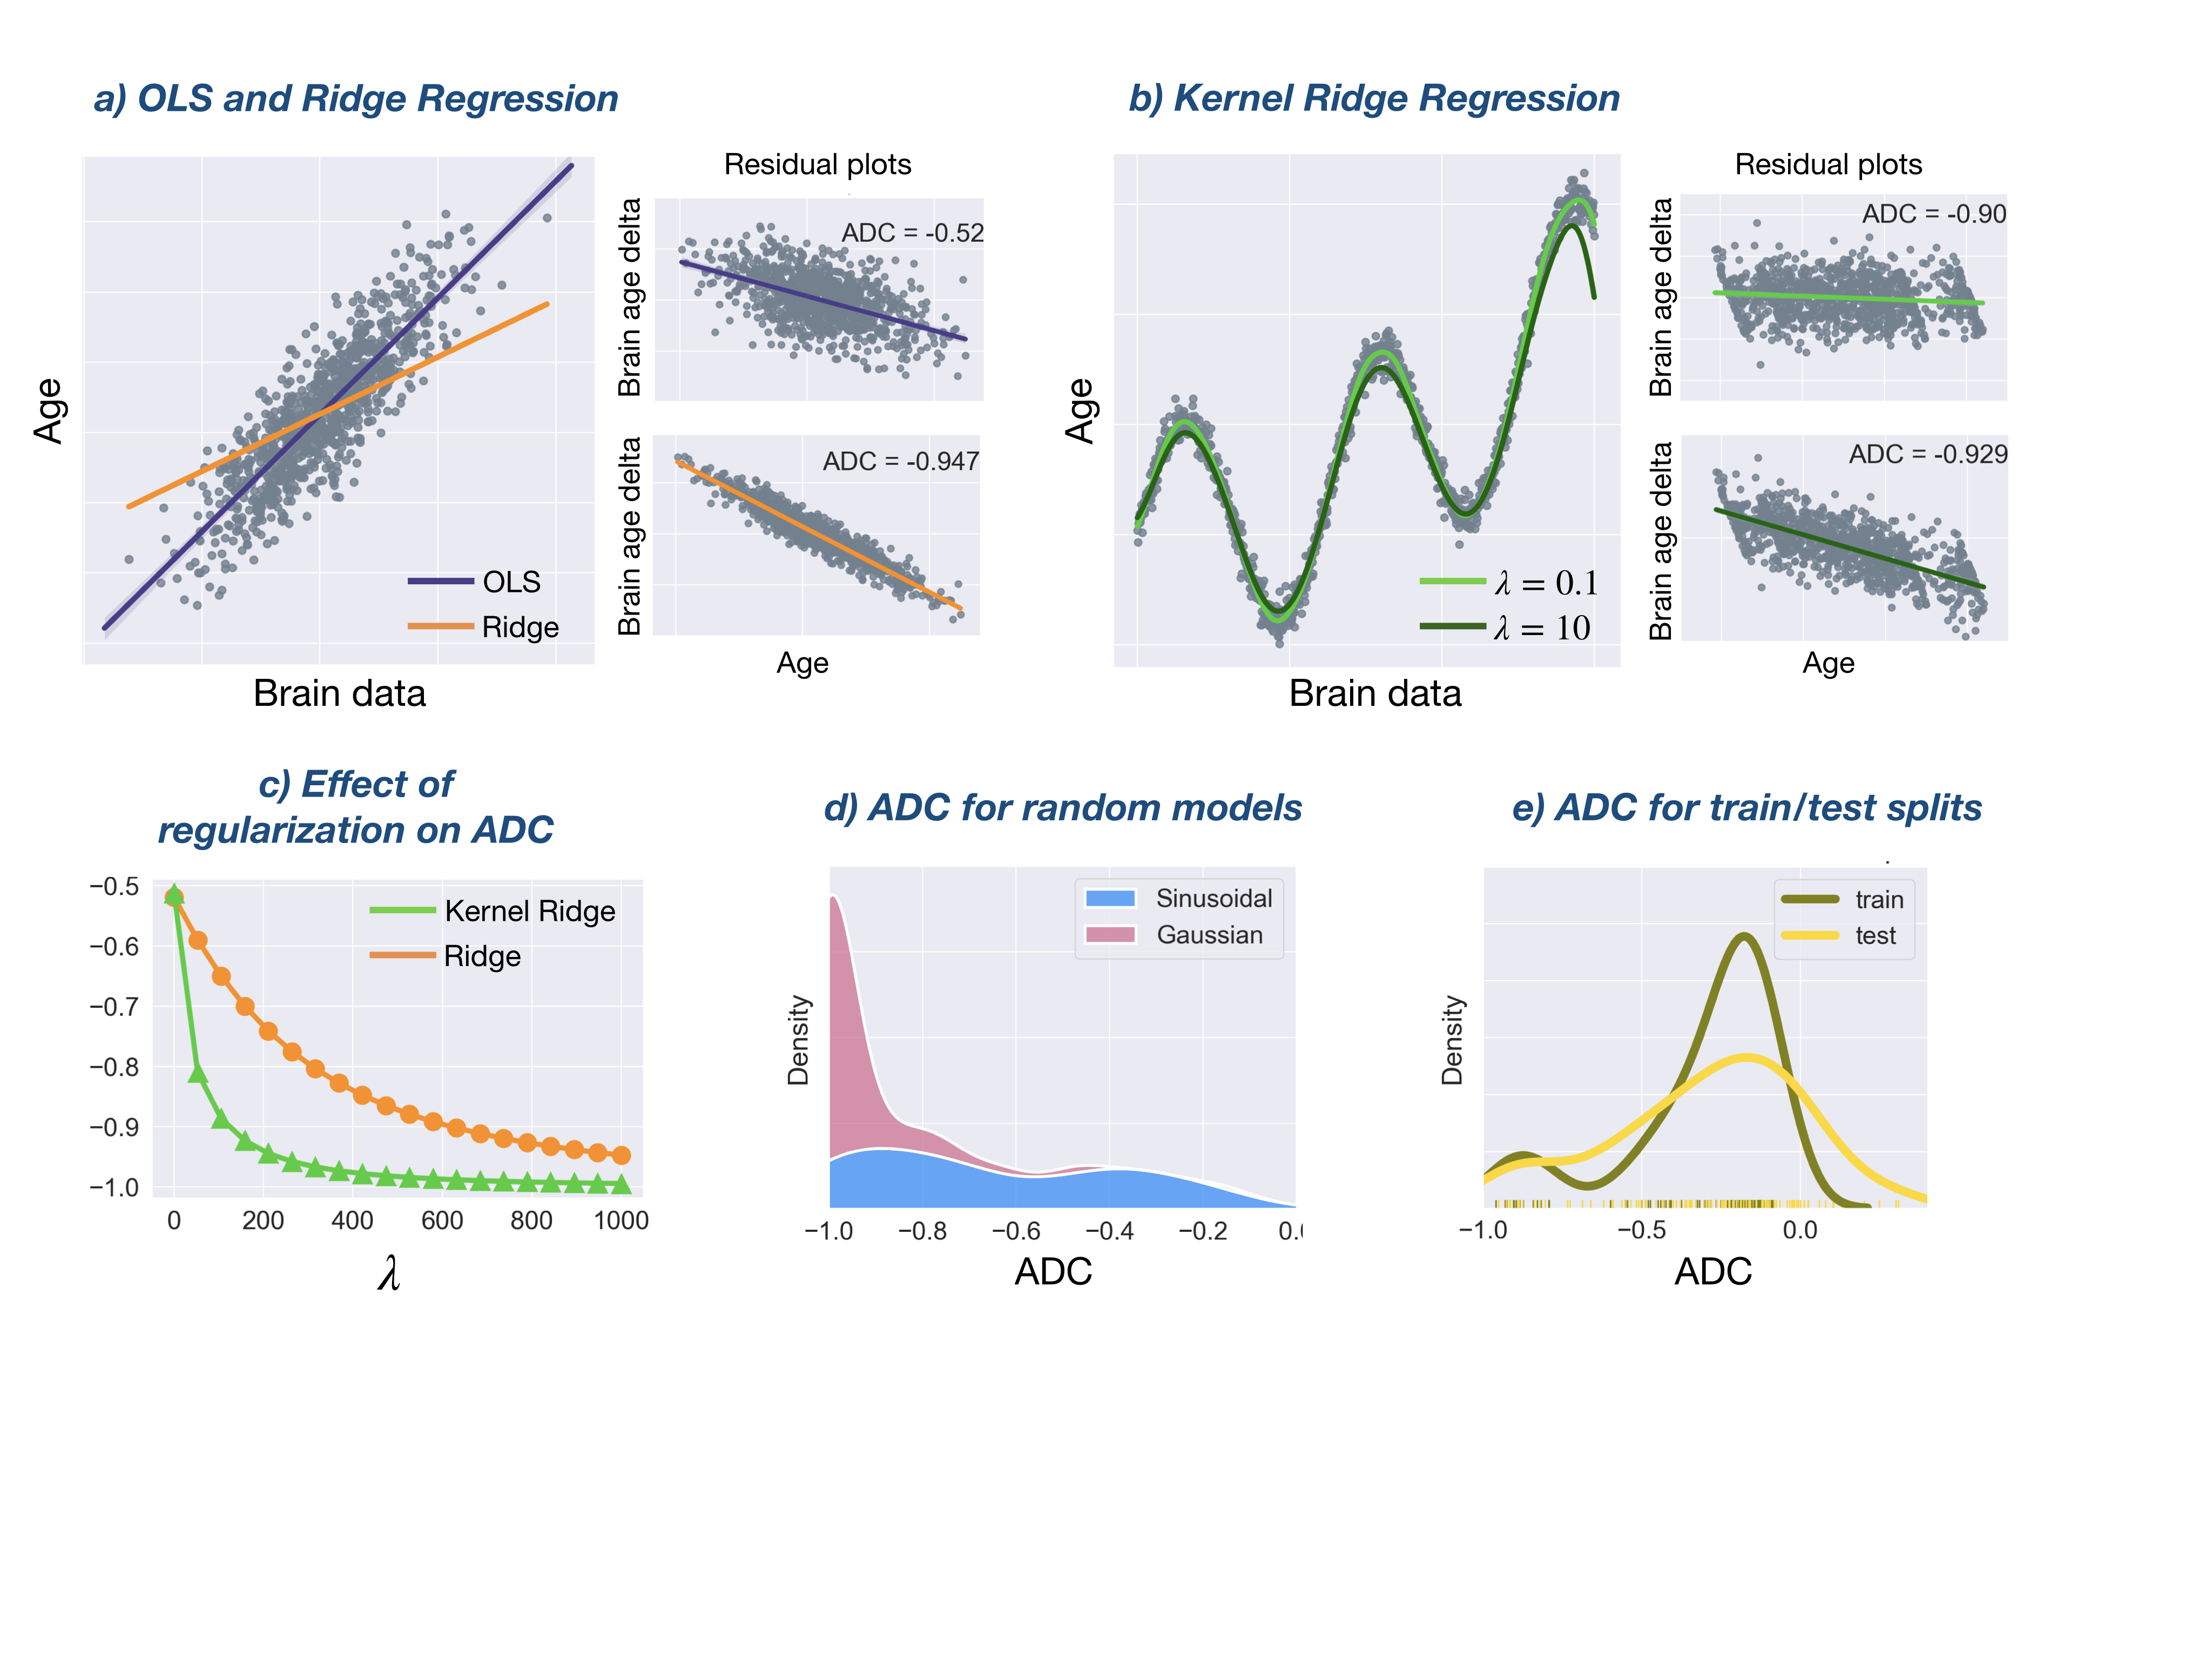
\includegraphics[width=1.\textwidth]{figures/ADC.jpeg}
\end{center}
\caption{Investigating age delta correlation (ADC)  with simulated data. \textbf{a)} Simulated data (1000 samples, 1 feature, linear function, Gaussian noise) using Scikit-Learn's make\_regression function. Regression line fits for OLS and Ridge ($\lambda=1000$) regression are shown. The small residual plots (plotting y vs residuals) show a significant negative ADC for both models. \textbf{b)} Simulated data (1000 samples, 1 feature, sine plus parabola function, Gaussian noise) with two Kernel Ridge regression fits (RBF kernel, $\gamma=1$) for two different regularization strengths $\lambda$. Again, residual plots show a high ADC. \textbf{c)} For both Ridge and Kernel Ridge regression, increasing the regularization hyperparameter $\lambda$ leads to higher ADC. This effect is more pronounced for Kernel Ridge than Ridge. \textbf{d)} ADC density plot. We sampled 100 random Gaussian and sine+parabola datasets as specified before. We created random regression models by  sampling slopes and intercepts from a uniform distribution (the sampling space included the OLS coefficients). When calculating ADCs on random models, a clear bias towards large negative ADC values is evident. \textbf{e)} ADC density plot. Simulated data (1000 samples, 5 features, linear function, Gaussian noise) is split into 50\% train, 50\% test data. An OLS model is calculated on the train data and ADC is calculated on both train and test data. For the test data, the variability of the ADC is larger than for train data, and its mode is slightly shifted towards a larger negative value.}\label{fig:ADC}
\end{figure}

\begin{figure}[h!]
\begin{center}
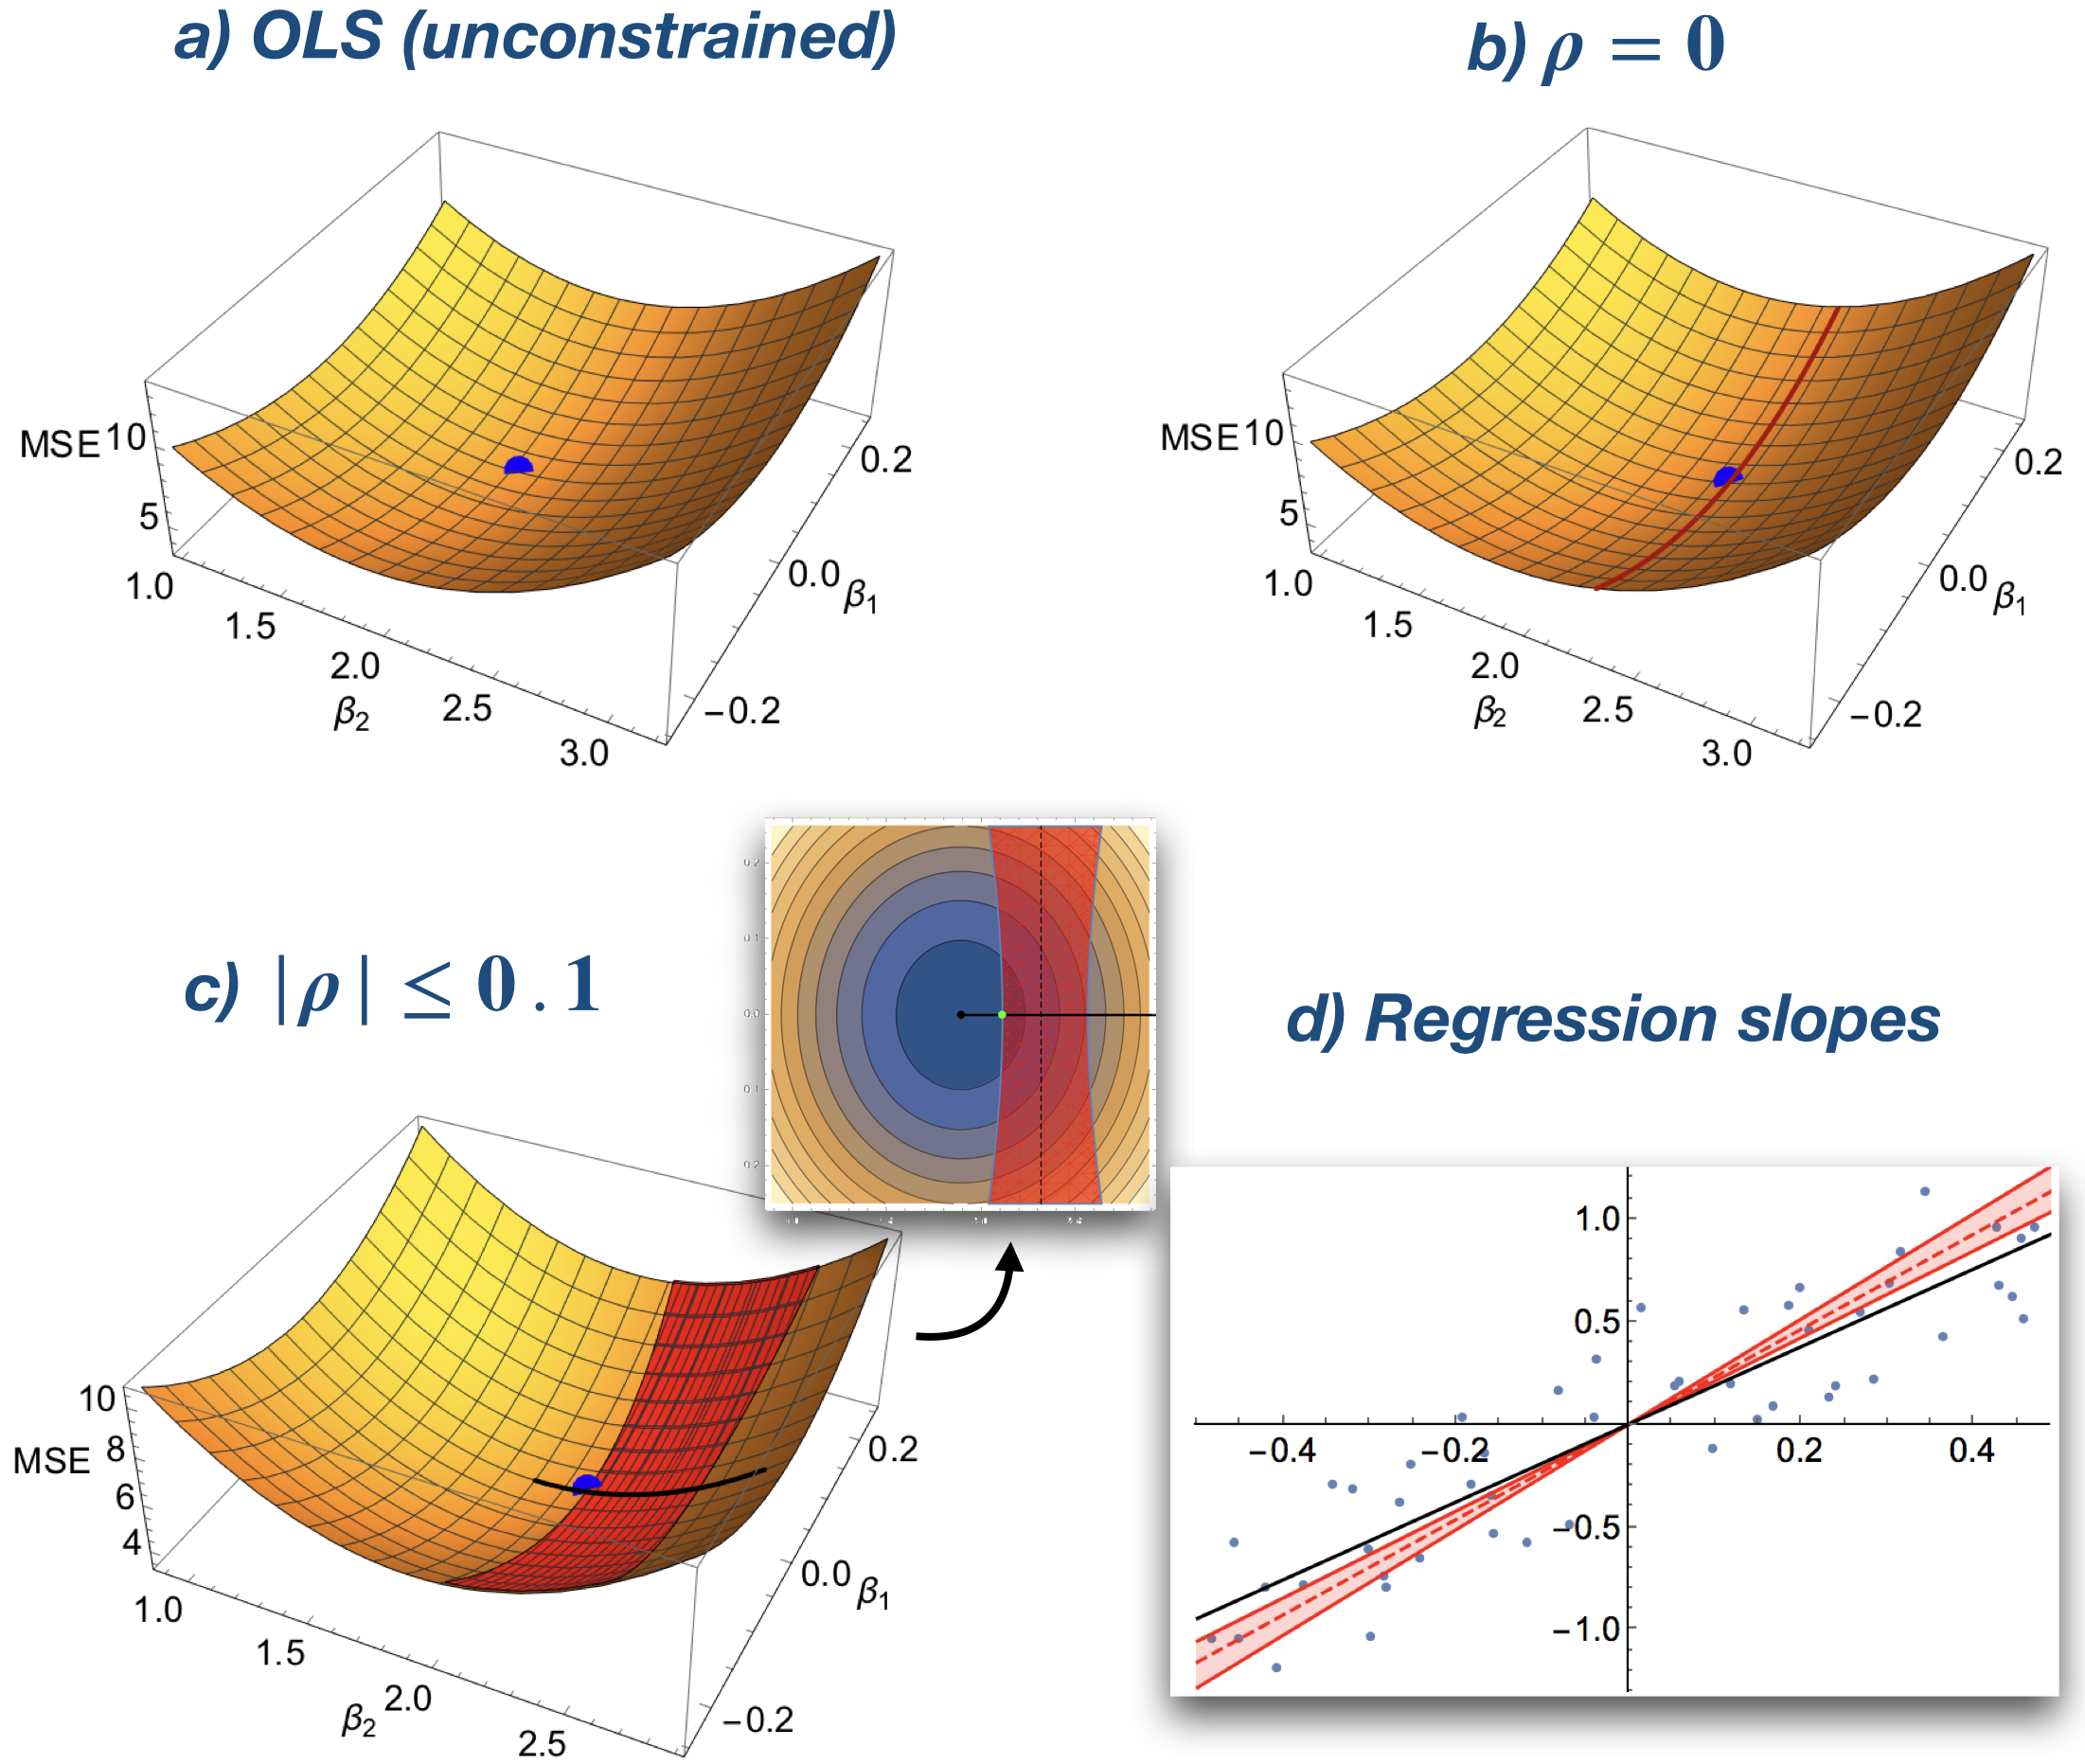
\includegraphics[width=1.\textwidth]{figures/geometrical_intuition.jpeg}
\end{center}
\caption{Geometrical intuition of optimization of an OLS model with correlation constraints. For illustrative purposes, simulated data is used with a model with two regression coefficients and without intercept. \textbf{a)} x and y axes represents different combinations of regression coefficients, whereas the z-axis represents the residual sum of squares. The standard unconstrained OLS fit corresponds to the minimum of the quadratic surface (blue ball). \textbf{b)} Zero correlation constraint. The solution space is restricted to a hyperplane (red line on the surface). The blue dot represents the optimal constrained solution. \textbf{c)} Bounded correlation. The solution space is restricted to the space between two paraboloids (red band on the surface). The inset depicts a 'top down' view on the surface. \textbf{d)} Corresponding regression slopes. The OLS solution is depicted as a black line. The correlation bound allows for a set of solutions (red shaded area) limited by $\rho=-0.1$ and $\rho=0.1$ (red solid lines). The zero ADC solution is depicted as a red dashed line.}\label{fig:geometrical_intuition}
\end{figure}


\begin{figure}[h!]
\begin{center}
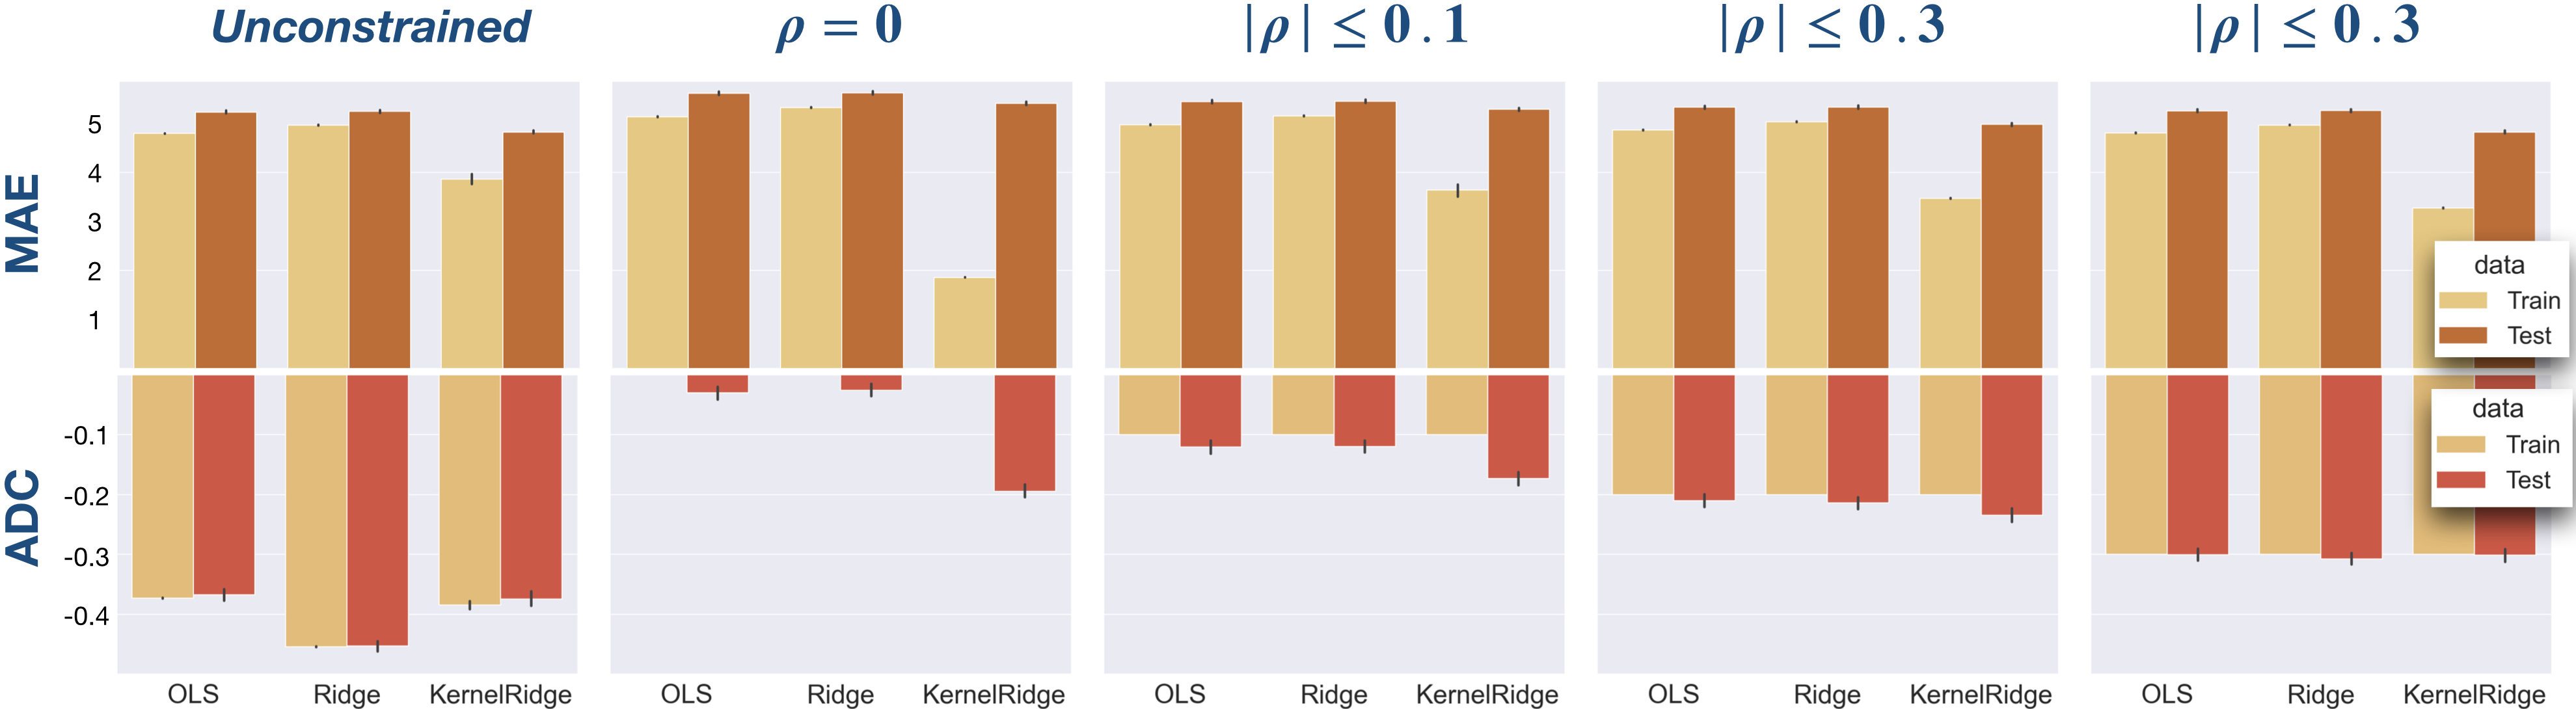
\includegraphics[width=1.\textwidth]{figures/Fig_PAC_Results.jpeg}
\end{center}
\caption{Analysis of PAC data using Linear Regression, Ridge, and Kernel Ridge regression models. \textbf{First row:} Mean absolute error (MAE) is depicted for the three different regression models and 5 different constraints: unconstrained (standard regression model), zero correlation constraint ($\rho=0$) and bounded correlation ($|\rho|\le0.1, 0.2, 0.3$). In terms of MAE, the best model on both train and test sets is Kernel Ridge regression.
\textbf{Second row:} ADC for different models and correlation constraints. Our models exactly control ADC on the training data and also reduce ADC on test data.}\label{fig:pac_results}
\end{figure}

\begin{figure}[h!]
\begin{center}
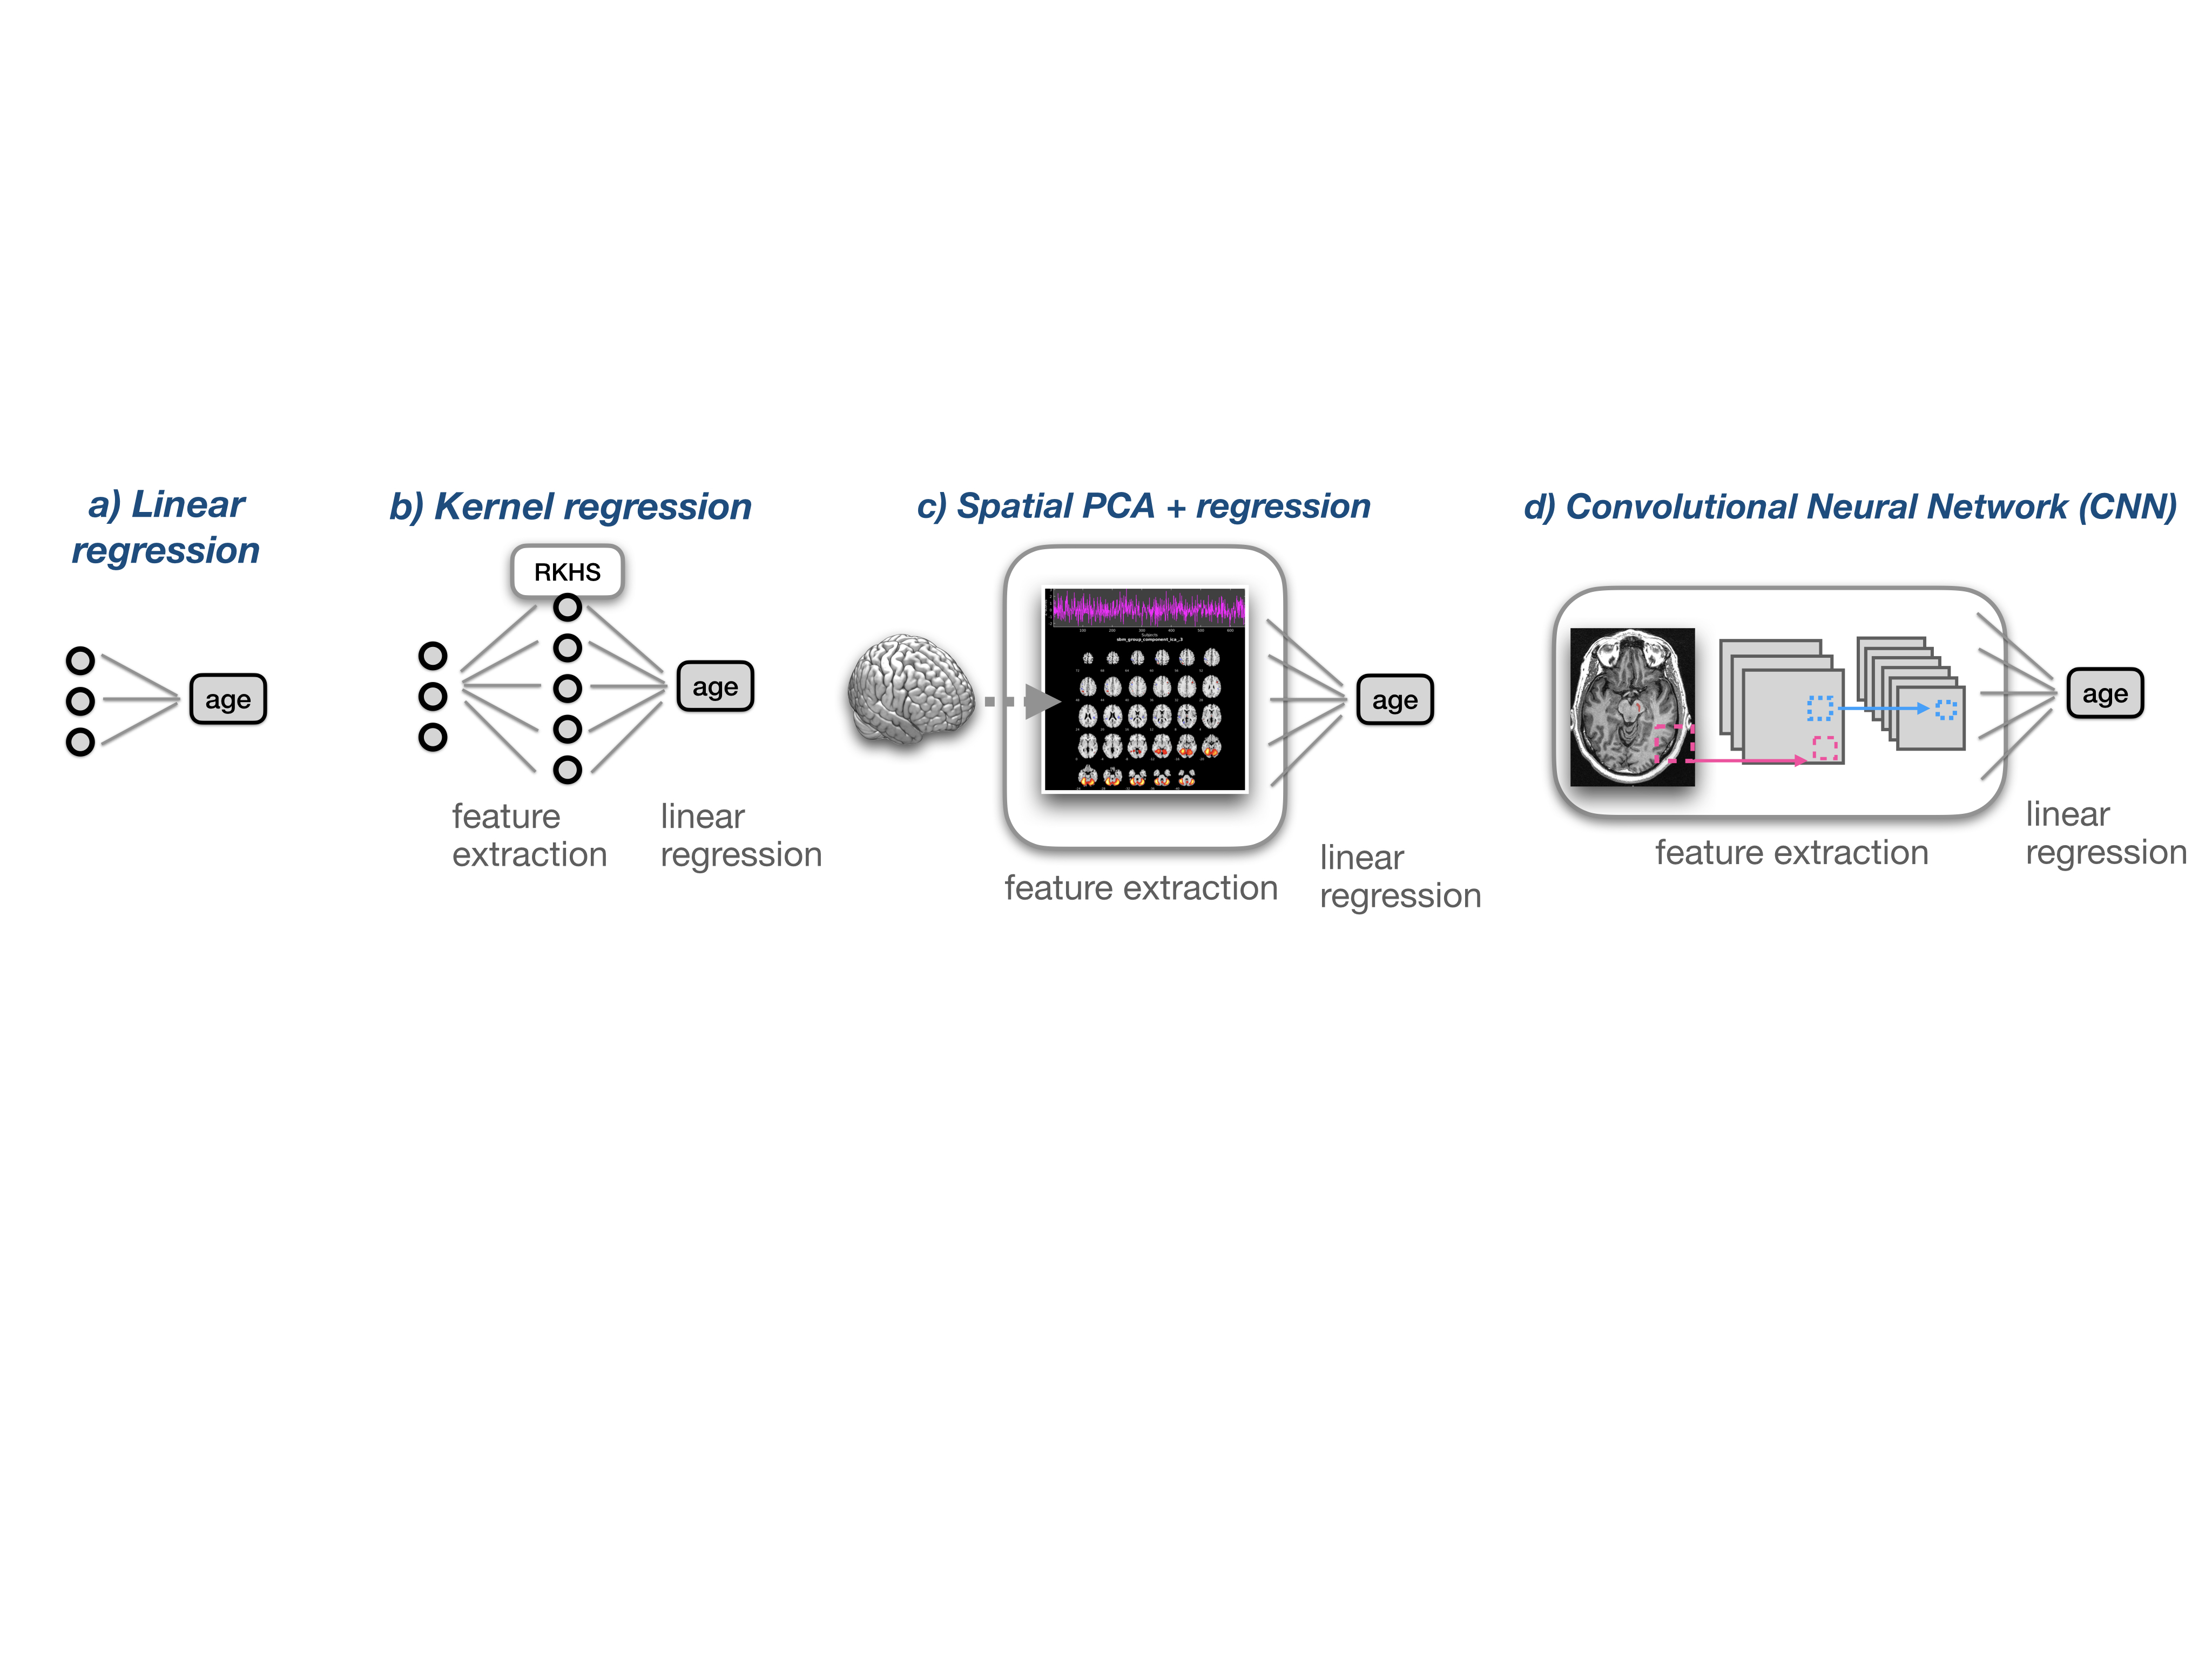
\includegraphics[width=1.\textwidth]{regression_models}
\end{center}
\caption{Coupled with non-linear feature extraction techniques, linear regression becomes a powerful model that is implicitly a part of many regression models. \textbf{a)} Linear regression using three features to predict age. \textbf{b)} Kernel regression can be conceived of as a projection of the data into a higher-dimensional, Reproducing Kernel Hilbert Space (RKHS), followed by linear regression in this space. \textbf{c)} MRIs can be transformed into components using PCA. For each MRI, its loadings on the different components can be used as features for linear regression. \textbf{d)} In Convolutional Neural Networks (CNN) for regression, the last layer is typically linear. The preceding layers can be conceived of as feature extraction layers, and the last layer performs linear regression on non-linear features.}\label{fig:regression_models}
\end{figure}


%%% If you are submitting a figure with subfigures please combine these into one image file with part labels integrated.
%%% If you don't add the figures in the LaTeX files, please upload them when submitting the article.
%%% Frontiers will add the figures at the end of the provisional pdf automatically
%%% The use of LaTeX coding to draw Diagrams/Figures/Structures should be avoided. They should be external callouts including graphics.

\end{document}
